\section{Auswertung}
\label{sec:Auswertung}
\subsection{Stehende Schallwellen}
\label{subsec:Stehende Schallwellen}
Abbildung \ref{fig:1-1} zeigt das Übersichtsspektrum des 600~mm langen Rohres von 0.1~kHz bis 10~kHz.
\begin{figure}
\centering
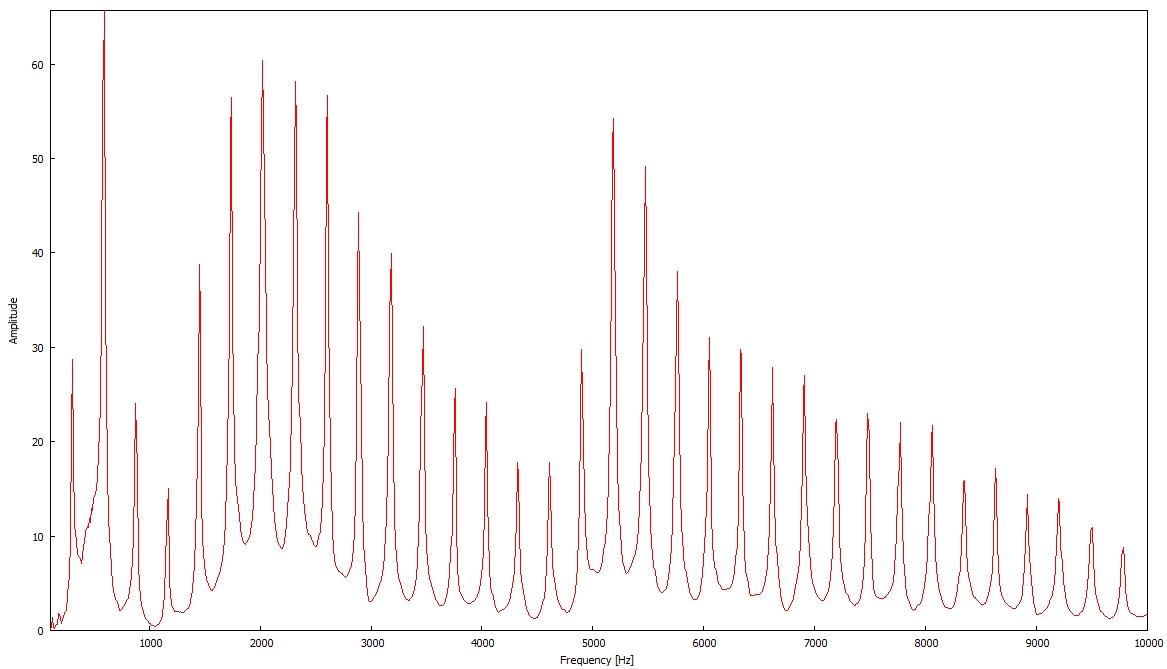
\includegraphics[width=\textwidth]{content/messungen/Chapter1/1-1img.jpg}
\caption{Übersichtsspektrum der Schallwellen in einem 600~mm langen Rohr von 0.1~kHz bis 10~kHz.}
\label{fig:1-1}
\end{figure}

Die zwei von 5~kHz bis 14~kHz aufgenommenen Spektren des 150~mm Rohres sind in den Abbildungen \ref{fig:1-2a:a} und \ref{fig:1-2b:a} dargestellt.
Zu diesen beiden Spektren sind die entsprechenden Fits in den Abbildungen \ref{fig:1-2a:b} und \ref{fig:1-2b:b} dargestellt.
Die vom Messprogramm ,,SpektrumSLC.exe'' erstellten Parameter, die die Peaks des Spektrums charakterisieren, sind in Tabelle \ref{tab:1:1} bzw. in Tabelle \ref{tab:1:2} aufgeführt.
Es zeigt sich an diesen beiden Tabellen, dass sich die Werte bis auf die Phase sehr gut reproduzieren lassen.
%%%%%%%%%%%%%%%%%%%%%%%%%%
\begin{figure}
\centering
\begin{subfigure}{0.4\textwidth}
\vspace{0.8cm}
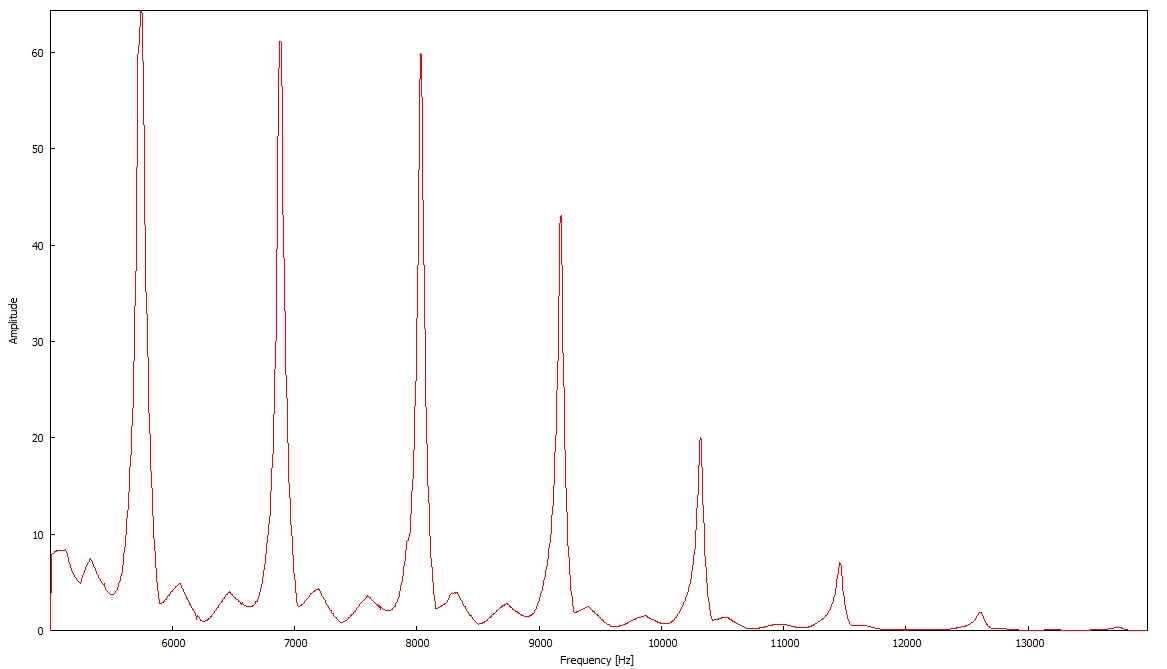
\includegraphics[width=\textwidth]{content/messungen/Chapter1/1-2img.jpg}
\subcaption{Rohdaten}
\label{fig:1-2a:a}
\end{subfigure}
\begin{subfigure}{0.4\textwidth}
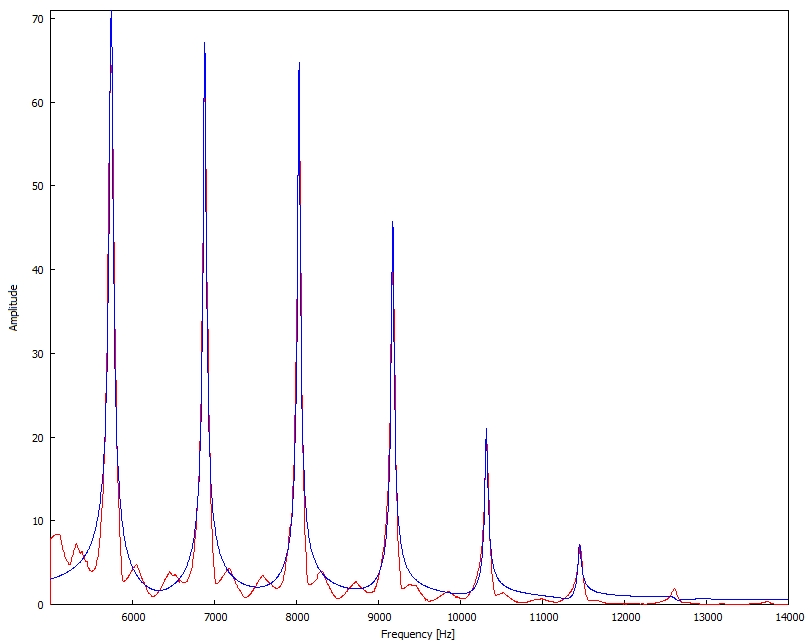
\includegraphics[width=\textwidth]{content/messungen/Chapter1/fit_img1.jpg}
\subcaption{Rohdaten mit Fit. Für Fitparameter siehe Tabelle \ref{tab:1:1}}
\label{fig:1-2a:b}
\end{subfigure}
\caption{Spektrum einer 150~mm langen Rühre von 5~kHz bis 14~kHz.}
\label{fig:1-2a}
\end{figure}
%%%%%%%%%%%%%%%%%%%%%%%%%%

%%%%%%%%%%%%%%%%%%%%%%%%%%
\begin{figure}
\centering
\begin{subfigure}{0.4\textwidth}
\vspace{0.8cm}
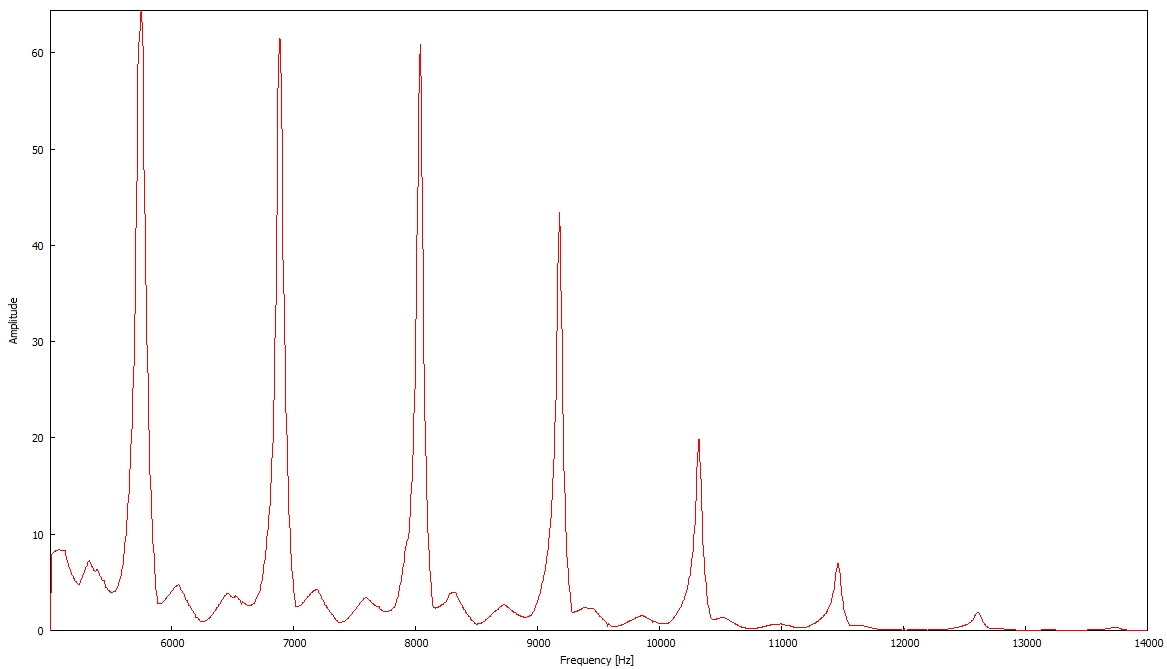
\includegraphics[width=\textwidth]{content/messungen/Chapter1/1-2-2img.jpg}
\subcaption{Rohdaten}
\label{fig:1-2b:a}
\end{subfigure}
\begin{subfigure}{0.4\textwidth}
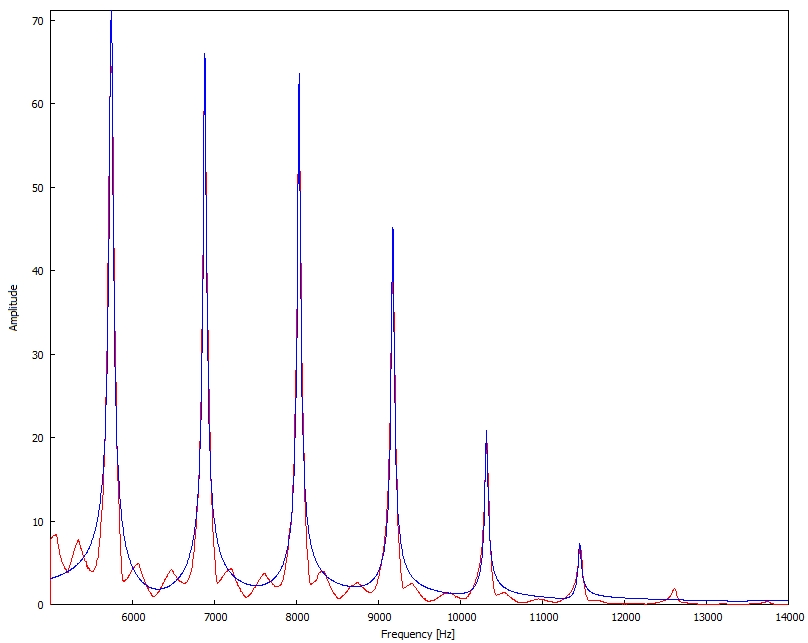
\includegraphics[width=\textwidth]{content/messungen/Chapter1/fit_img2.jpg}
\subcaption{Rohdaten mit Fit. Für Fitparameter siehe Tabelle \ref{tab:1:1}}
\label{fig:1-2b:b}
\end{subfigure}
\caption{Wiederholungsmessung des Spektrums einer 150~mm langen Rühre von 5~kHz bis 14~kHz.}
\label{fig:1-2b}
\end{figure}
%%%%%%%%%%%%%%%%%%%%%%%%%%

\begin{table}
\centering
\caption{Ergebnis des Fits aus Abbildung \ref{fig:1-2a}.}
\label{tab:1:1}
\begin{tabular}{c c c c c c c c c}
\hline
 & Peak 1 & Peak 2 & Peak 3 & Peak 4 & Peak 5 & Peak 6&Peak 7&Peak 8 \\ \hline

Frequenz in Hz& 5750&6890&8030&9180&10300&11500&12600&17200\\
Amplitude&69.9&65.8&63.5&44.6&20.0&6.45&0.41&0.20\\
Breite in Hz&21.3&16.6&14.6&15.0&16.2&20.1&52.1&4200\\
Phase in Grad&-51.0&-31.2&4.3&38.2&57.5&50.5&-140&178\\
\hline
\end{tabular}
\end{table}

\begin{table}
\centering
\caption{Ergebnis des Fits aus Abbildung \ref{fig:1-2b}.}
\label{tab:1:2}
\begin{tabular}{c c c c c c c c c}
\hline
 & Peak 1 & Peak 2 & Peak 3 & Peak 4 & Peak 5 & Peak 6&Peak 7&Peak 8 \\ \hline

Frequenz in Hz&5750&6890&8030&9180&10300&11500&13500&13700\\
Amplitude&70.0&64.8&62.0&44.1&19.9&6.60&0.02&0.18\\
Breite in Hz&21.3&17.5&15.8&15.6&16.2&18.2&512&230\\
Phase in Grad&-46.5&-26.1&9.90&51.2&72.3&72.5&-107&37.0\\
\hline
\end{tabular}
\end{table}
\FloatBarrier
\subsection{Der Kugelresonator}
\label{subsec:Der Kugelresonator}
Die Übersichtsspektren für die Winkel $\alpha=0\degree,30\degree,60\degree,90\degree,120\degree,150\degree,180\degree$ werden in den Abbildung \ref{fig:2_1_0} bis \ref{fig:2_1_180} dargestellt.
%%%%%%%%%%%%%%%%%%%%%%%%
\begin{figure}
\centering
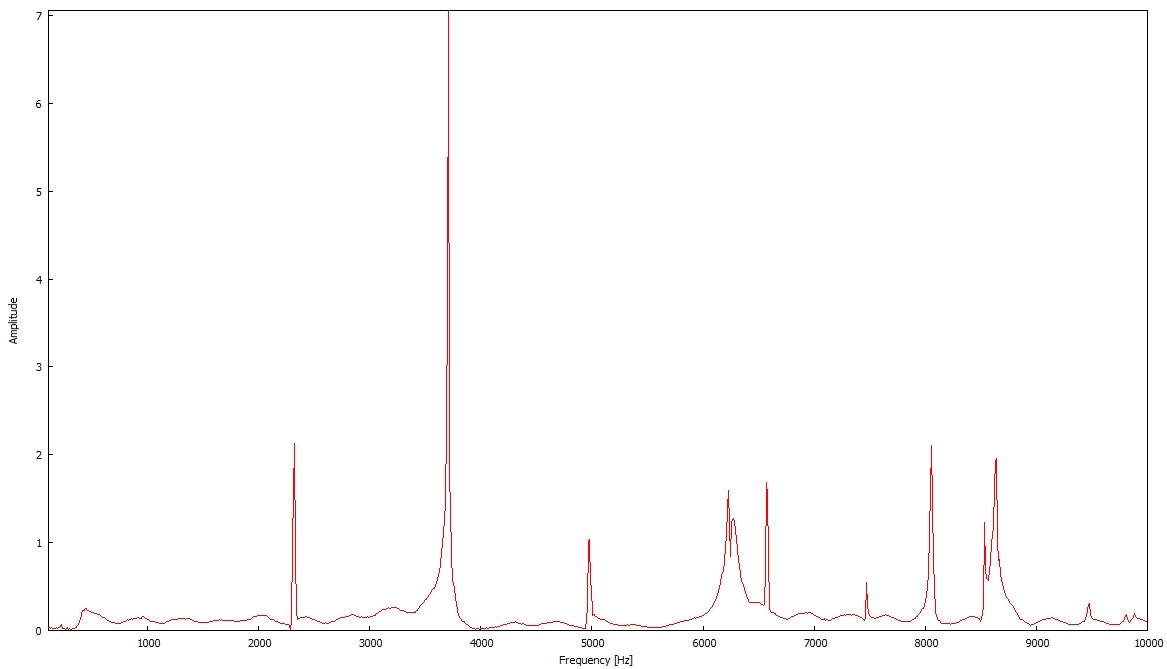
\includegraphics[width=\textwidth]{content/messungen/Chapter2new/2_1_0img.jpg}
\caption{Übersichtsspektrum des Kugelresonators von 0.1~kHz bis 10~kHz für $\alpha=0\degree$.}
\label{fig:2_1_0}
\end{figure}

\begin{figure}
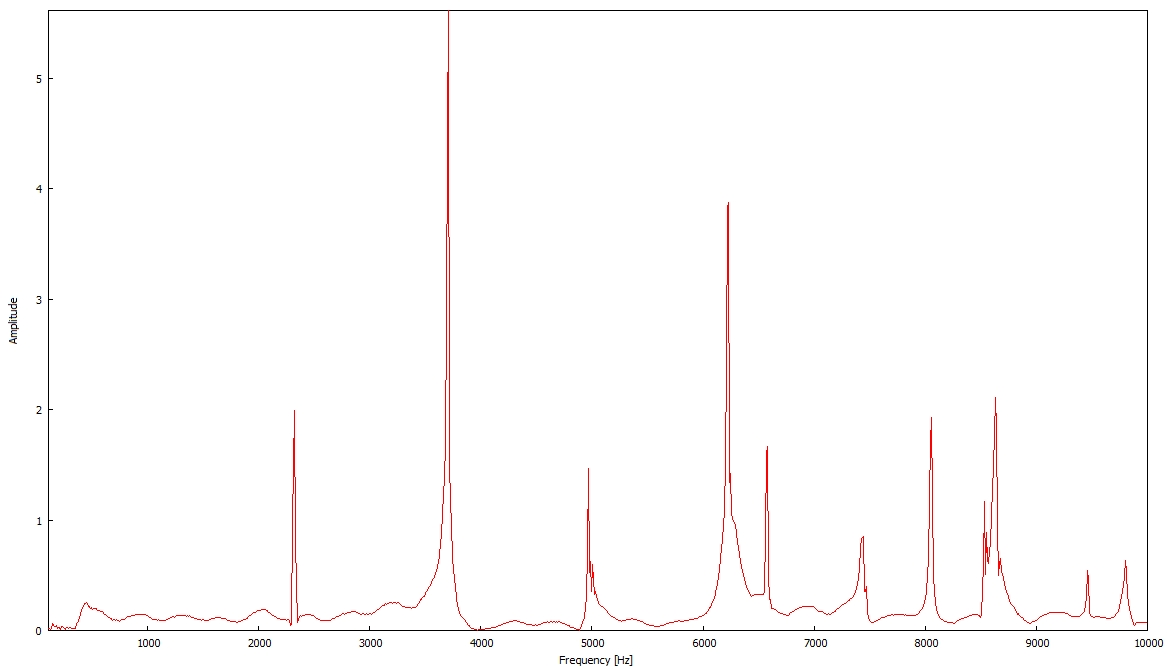
\includegraphics[width=\textwidth]{content/messungen/Chapter2new/2_1_30img.jpg}
\caption{Übersichtsspektrum des Kugelresonators von 0.1~kHz bis 10~kHz für $\alpha=30\degree$.}
\label{fig:2_1_30}
\end{figure}

\begin{figure}
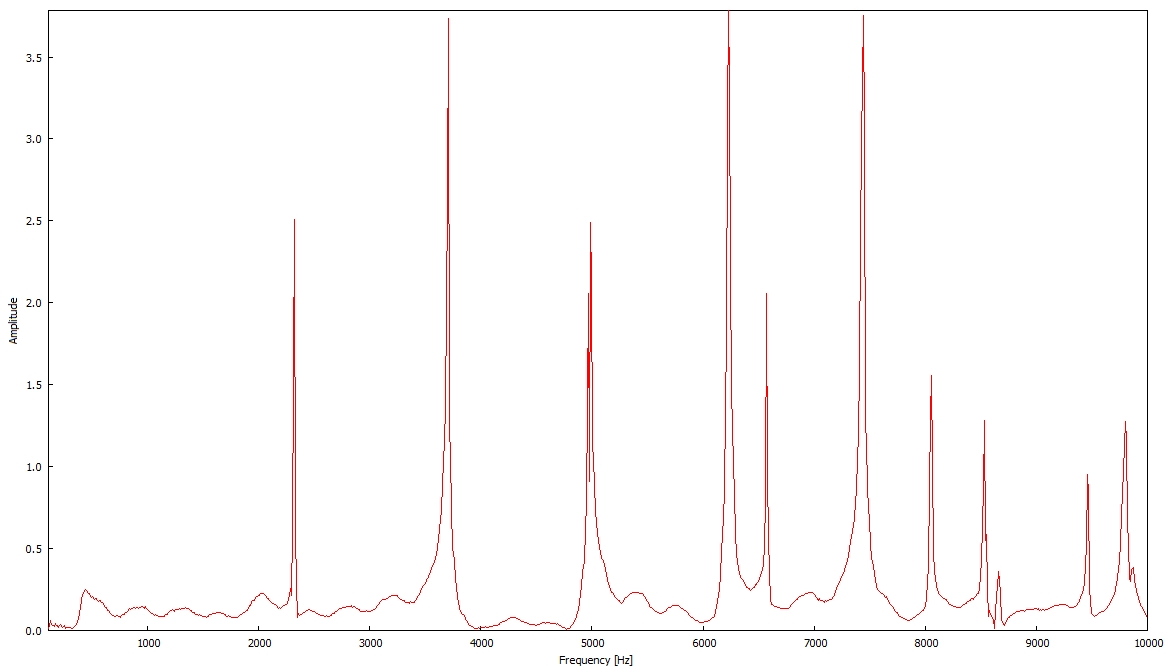
\includegraphics[width=\textwidth]{content/messungen/Chapter2new/2_1_60img.jpg}
\caption{Übersichtsspektrum des Kugelresonators von 0.1~kHz bis 10~kHz für $\alpha=60\degree$.}
\label{fig:2_1_60}
\end{figure}

\begin{figure}
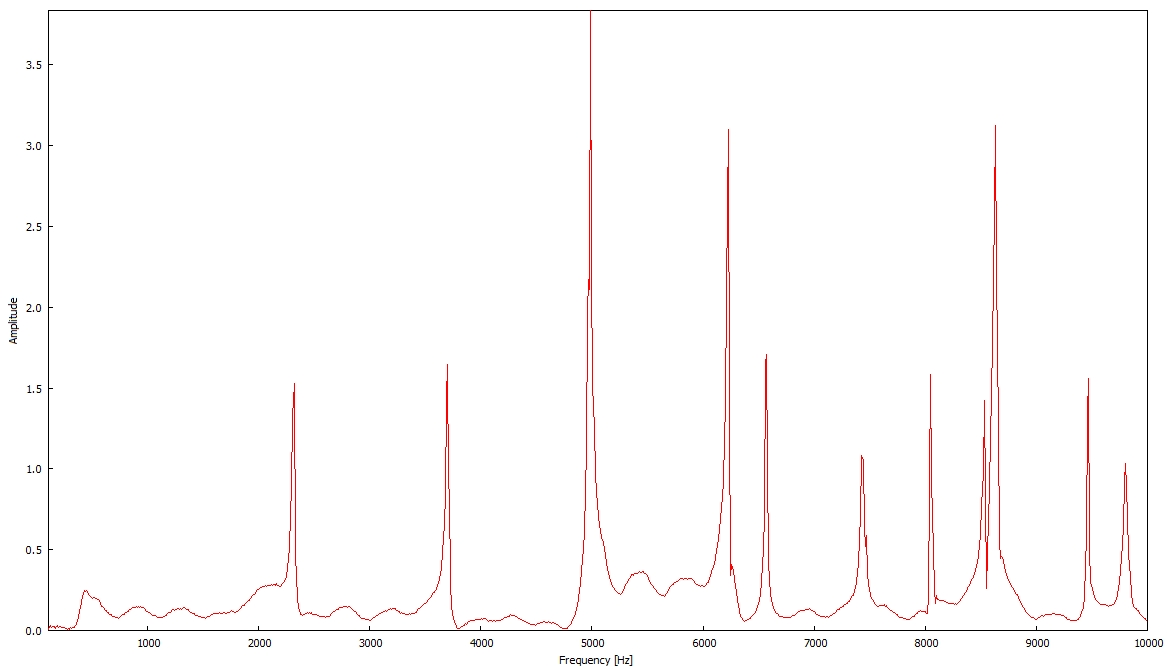
\includegraphics[width=\textwidth]{content/messungen/Chapter2new/2_1_90img.jpg}
\caption{Übersichtsspektrum des Kugelresonators von 0.1~kHz bis 10~kHz für $\alpha=90\degree$.}
\label{fig:2_1_90}
\end{figure}

\begin{figure}
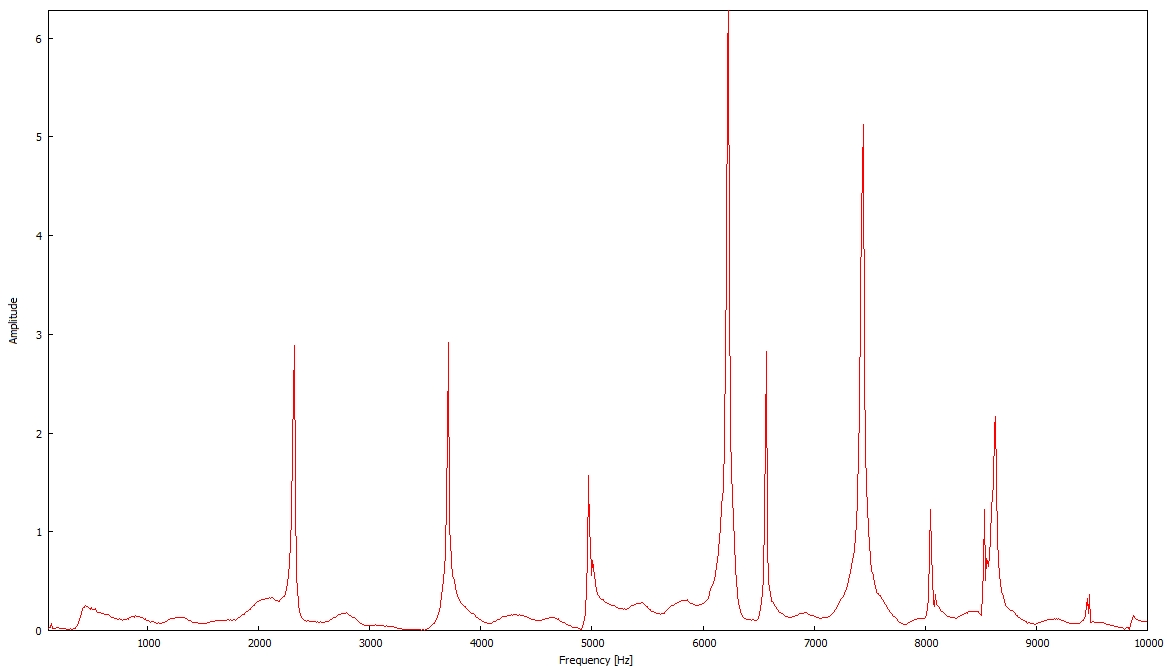
\includegraphics[width=\textwidth]{content/messungen/Chapter2new/2_1_120img.jpg}
\caption{Übersichtsspektrum des Kugelresonators von 0.1~kHz bis 10~kHz für $\alpha=120\degree$.}
\label{fig:2_1_120}
\end{figure}

\begin{figure}
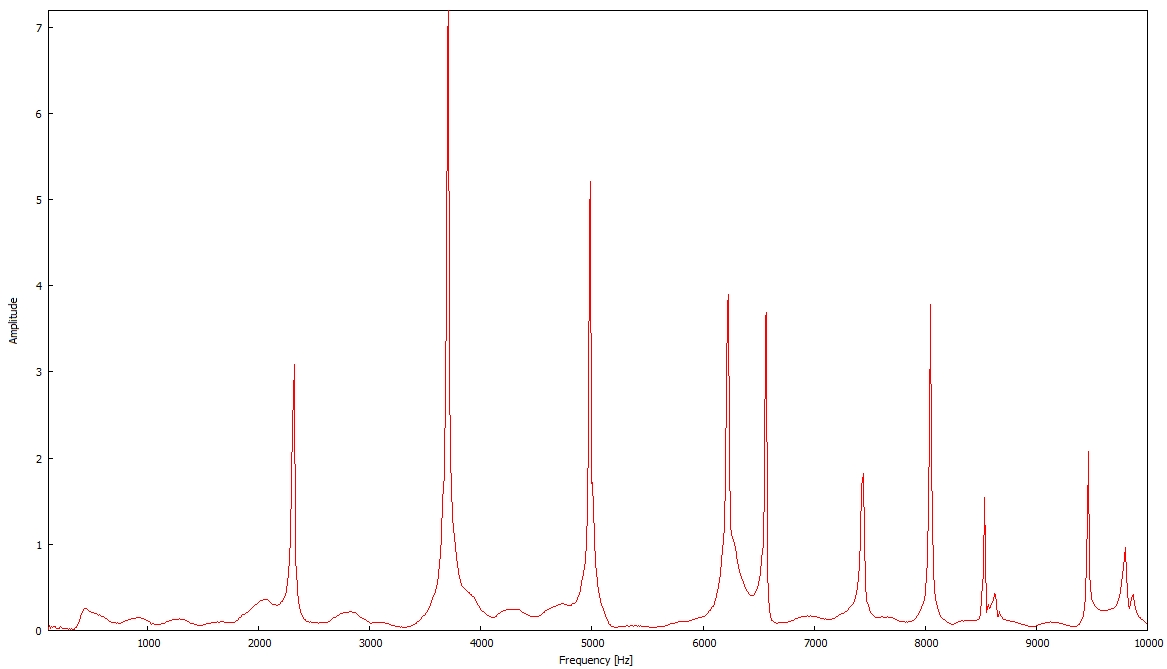
\includegraphics[width=\textwidth]{content/messungen/Chapter2new/2_1_150img.jpg}
\caption{Übersichtsspektrum des Kugelresonators von 0.1~kHz bis 10~kHz für $\alpha=150\degree$.}
\label{fig:2_1_150}
\end{figure}

\begin{figure}
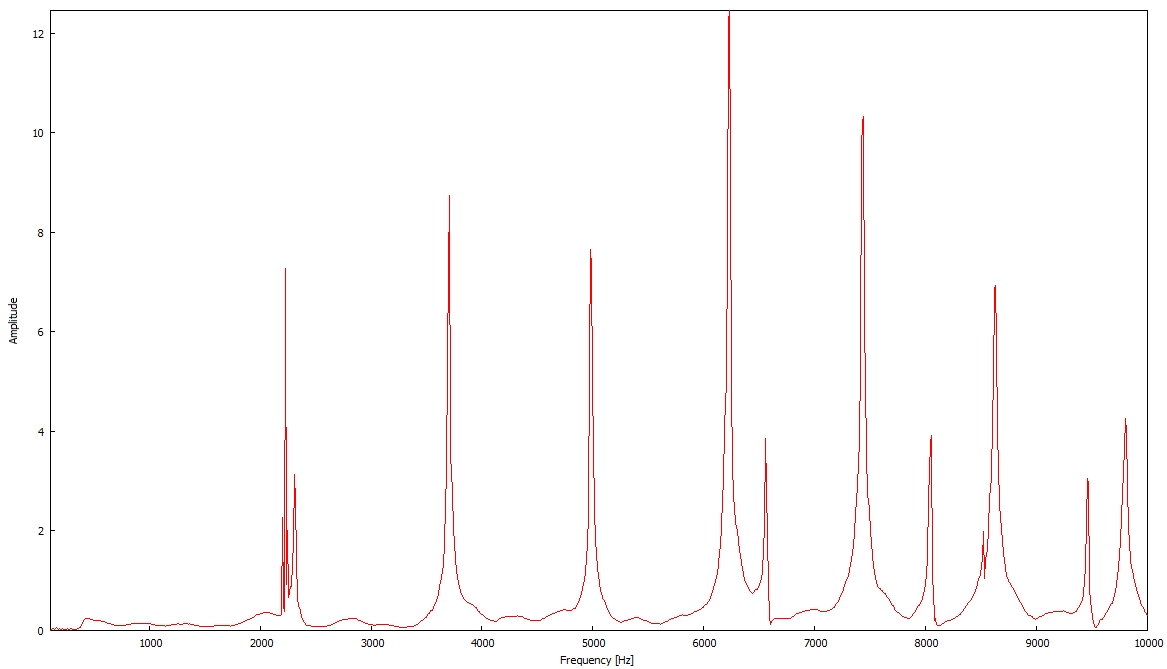
\includegraphics[width=\textwidth]{content/messungen/Chapter2new/2_1_180img.jpg}
\caption{Übersichtsspektrum des Kugelresonators von 0.1~kHz bis 10~kHz für $\alpha=180\degree$.}
\label{fig:2_1_180}
\end{figure}
%%%%%%%%%%%%%%%%%%%%%%%%%%%%%
An ihnen ist zu erkennen, dass die Resonanzen für alle $\alpha$ an den selben Stellen liegen. 
Lediglich die Amplitude variiert.
Die Abbildungen \ref{fig:2_2_0} bis \ref{fig:2_2_40} zeigen die Untersuchungsergebnisse der Resonanzstelle bei ca. 5~kHz. 
\begin{figure}
\centering
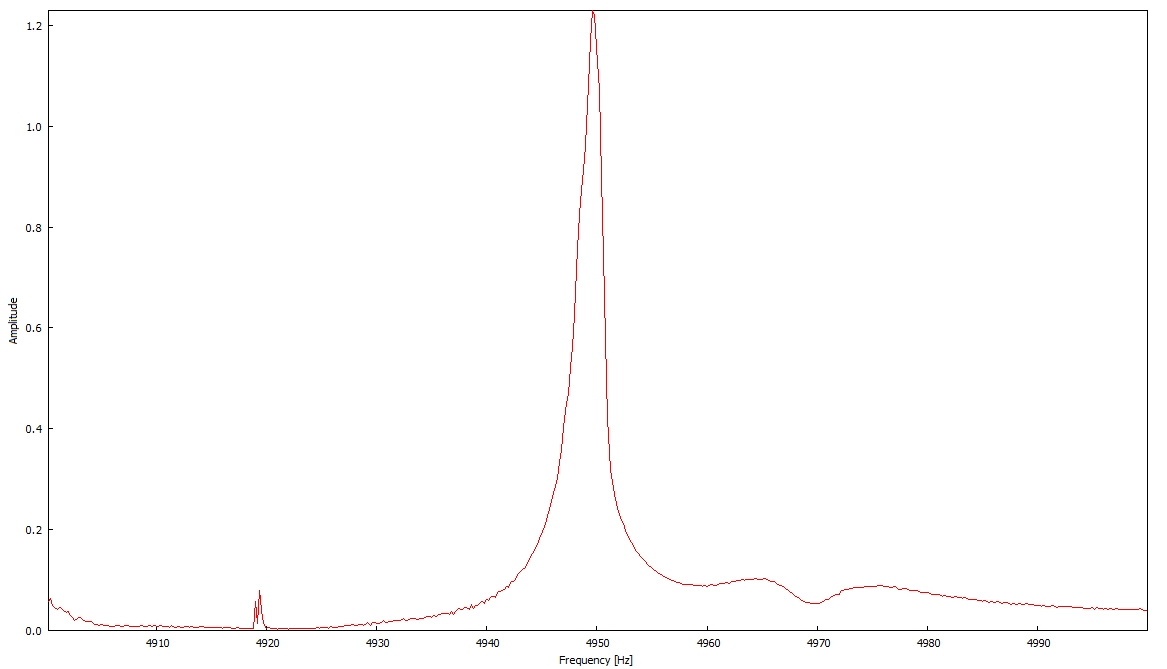
\includegraphics[width=\textwidth]{content/messungen/Chapter2new/2_2_0img.jpg}
\caption{Die dritte Resonanzstelle des Kugelresonators wird für $\alpha=0\degree$ zwischen 4.9~kHz und 5.0~kHz untersucht.}
\label{fig:2_2_0}
\end{figure}
\begin{figure}
\centering
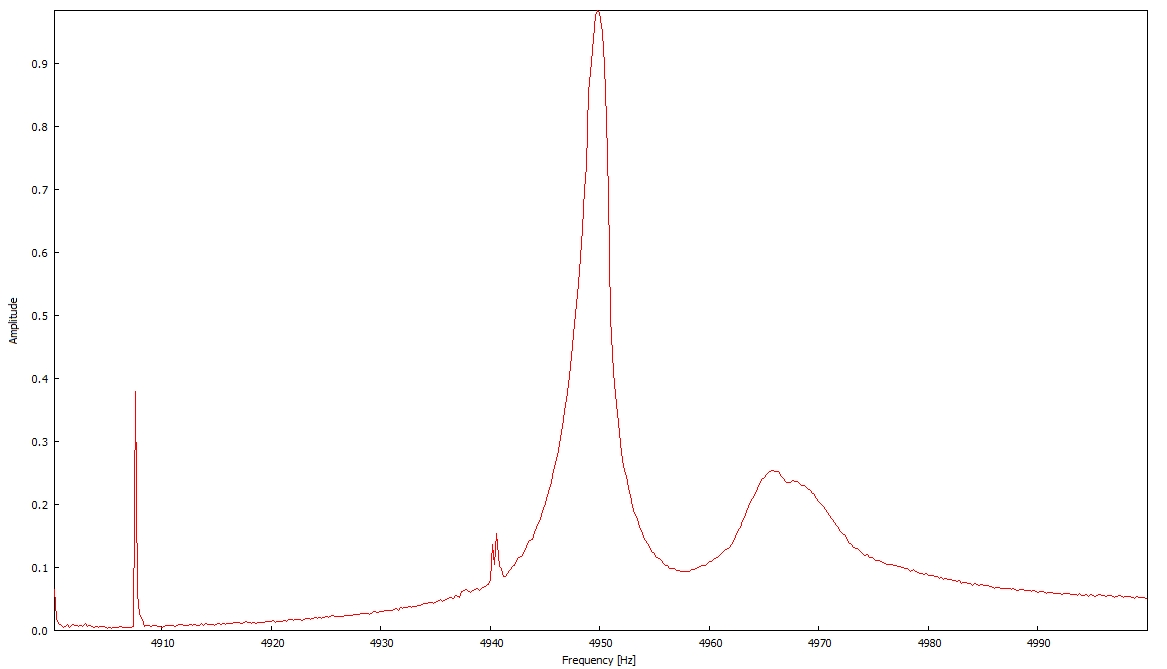
\includegraphics[width=\textwidth]{content/messungen/Chapter2new/2_2_20mg.jpg}
\caption{Die dritte Resonanzstelle des Kugelresonators wird für $\alpha=20\degree$ zwischen 4.9~kHz und 5.0~kHz untersucht.}
\label{fig:2_2_20}
\end{figure}
\begin{figure}
\centering
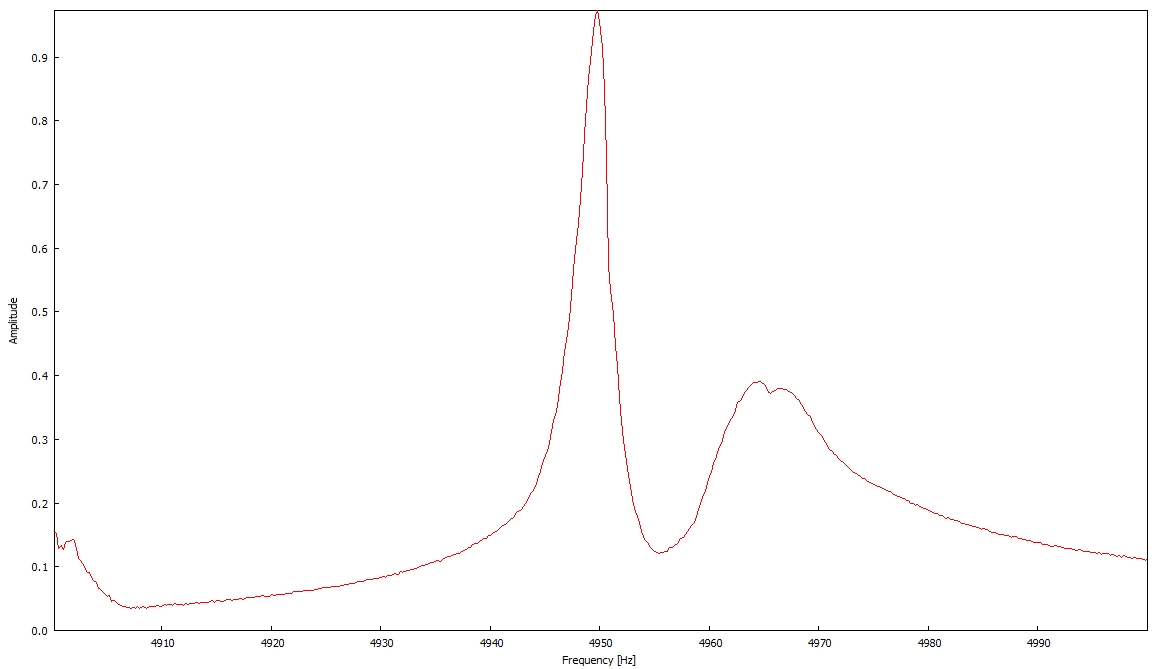
\includegraphics[width=\textwidth]{content/messungen/Chapter2new/2_2_40mg.jpg}
\caption{Die dritte Resonanzstelle des Kugelresonators wird für $\alpha=40\degree$ zwischen 4.9~kHz und 5.0~kHz untersucht.}
\label{fig:2_2_40}
\end{figure}
Um nun die Messungen an festen Resonanzstellen darzustellen wird das in Abbildung \ref{fig:2_3_180} aufgeführte von 2~kHz bis 7~kHz aufgenommene Spektrum betrachtet.
\begin{figure}
\centering
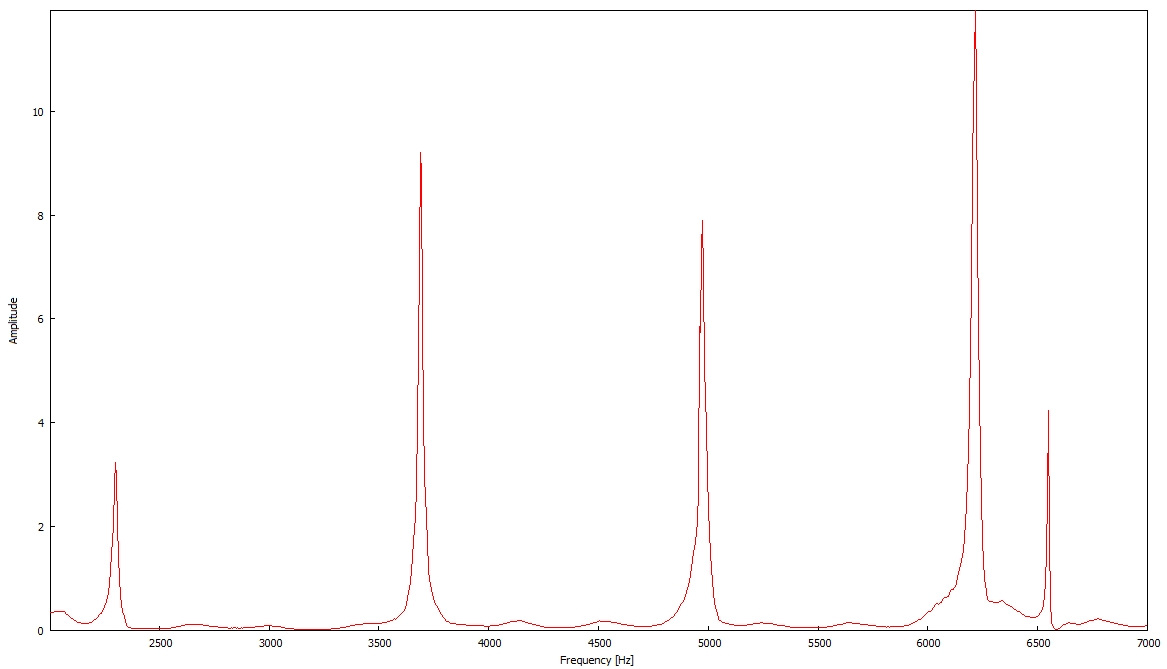
\includegraphics[width=\textwidth]{content/messungen/Chapter2new/2_3_180mg.jpg}
\caption{Spektrum des Kugelresonators von 2~kHz bis 7~kHz bei $\alpha=180\degree$.}
\label{fig:2_3_180}
\end{figure}
Die fünf zu erkennenden Resonanzstellen werden bei fester Frequenz durch variieren des Winkels $\alpha$ ausgemessen.
Es sei darauf hingewiesen, dass der Computer $\alpha$ automatisch in die gesuchte Größte $\theta$ umrechnet.
Um der Symmetrie des Kugelresonators gerecht zu werden, werden die Ergebnisse in den Polarplots \ref{fig:2_3_1} bis \ref{fig:2_3_5} dargestellt.
%%%%%%%%%%%%%%%%%%%%
\begin{figure}
\centering
\begin{subfigure}{0.4\textwidth}
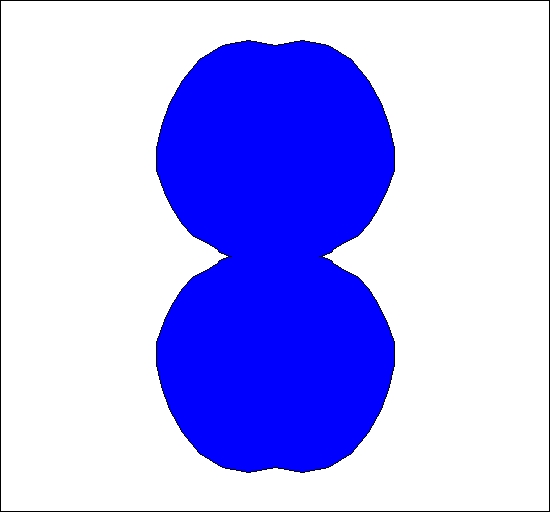
\includegraphics[width=\textwidth]{content/messungen/Chapter2new/2_3_1.jpg}
\subcaption{Frequenz ca. 2.30~kHz, $m=0, l=1$.}
\label{fig:2_3_1}
\end{subfigure}
\begin{subfigure}{0.4\textwidth}
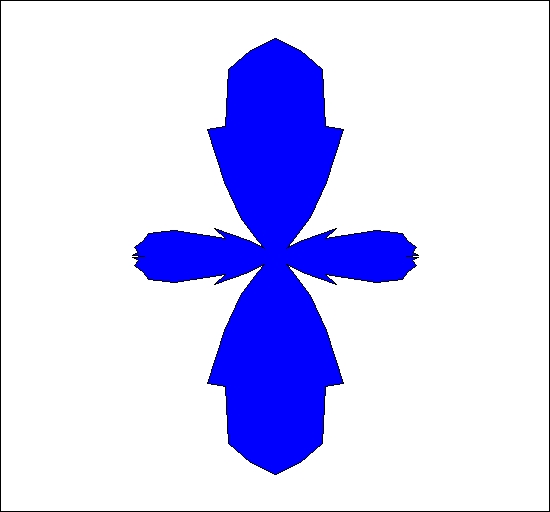
\includegraphics[width=\textwidth]{content/messungen/Chapter2new/2_3_2.jpg}
\subcaption{Frequenz ca. 3.69~kHz, $m=0, l=2$.}
\label{fig:2_3_2}
\end{subfigure}

\begin{subfigure}{0.4\textwidth}
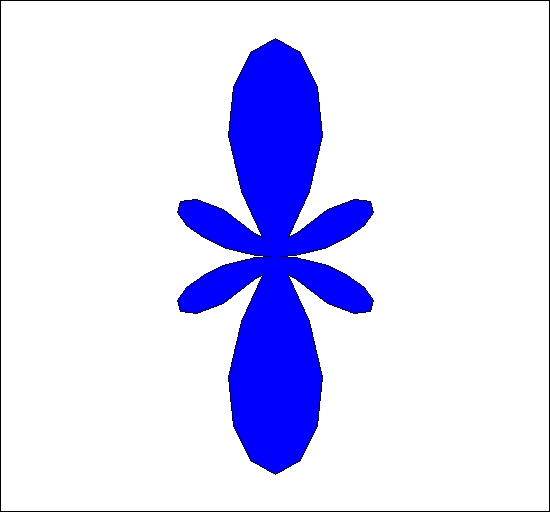
\includegraphics[width=\textwidth]{content/messungen/Chapter2new/2_3_3.jpg}
\subcaption{Frequenz ca. 4.98~kHz, $m=0, l=3$.}
\label{fig:2_3_3}
\end{subfigure}
\begin{subfigure}{0.4\textwidth}
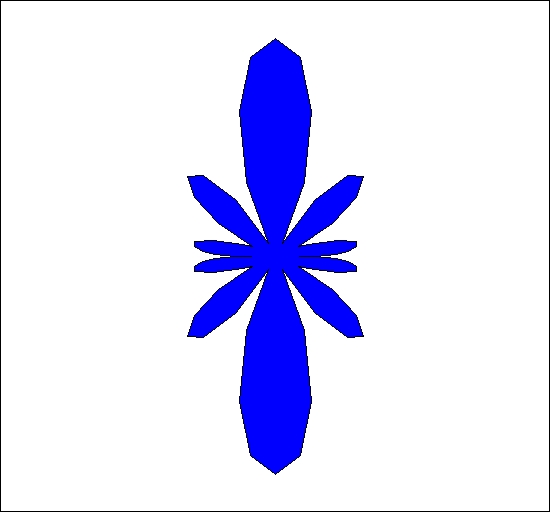
\includegraphics[width=\textwidth]{content/messungen/Chapter2new/2_3_4.jpg}
\subcaption{Frequenz ca. 6.21~kHze, $m=0, l=5$.}
\label{fig:2_3_4}
\end{subfigure}

\begin{subfigure}{0.4\textwidth}
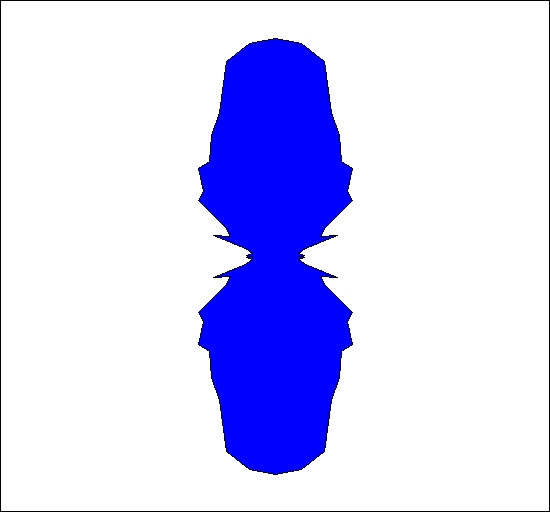
\includegraphics[width=\textwidth]{content/messungen/Chapter2new/2_3_5.jpg}
\subcaption{Frequenz ca. 6.55~kHz, $m=0, l=1$.}
\label{fig:2_3_5}
\end{subfigure}
\caption{Schallamplitude im Kugelresonator in Abhängigkeit des Winkels $\theta$ und zugehörige Quantenzahlen.}
\label{fig:kugelflaechenfunktionen}
\end{figure}
%%%%%%%%%%%%%%%%%%%%%
\FloatBarrier
\subsection{Modell eines eindimensionalen Festkörpers}
\label{subsec:Modell eines eindimensionalen Festkörpers}
Die im Bereich zwischen 5~kHz und 9~kHz aufgenommenen Spektren der verschieden langen Rohre sind in den Abbildungen \ref{fig:4_1_75} bis \ref{fig:4_1_600} dargestellt.
Die Messung zeigt eine höhere Dichte der Resonanzen bei zunehmender Rohrlänge.
\begin{figure}
\centering
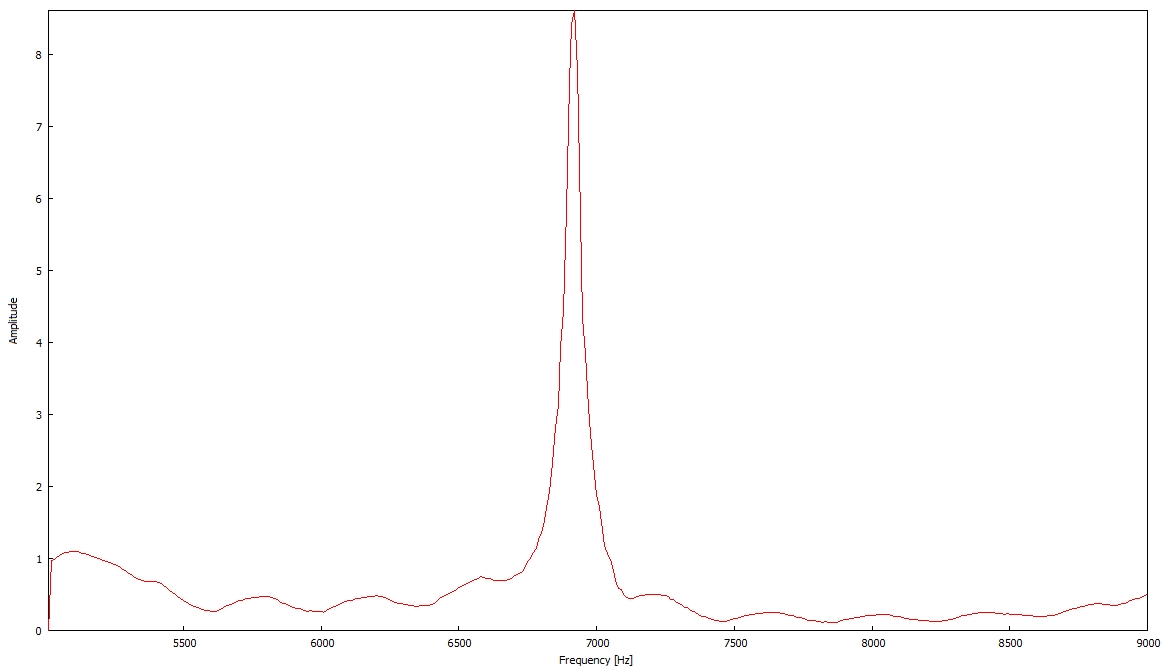
\includegraphics[width=1\textwidth]{content/messungen/Chapter4/4_1_75mm.jpg}
\caption{Spektrum eines 75~mm langen Rohres zwischen 5~kHz und 9~kHz.}
\label{fig:4_1_75}
\end{figure}

\begin{figure}
\centering
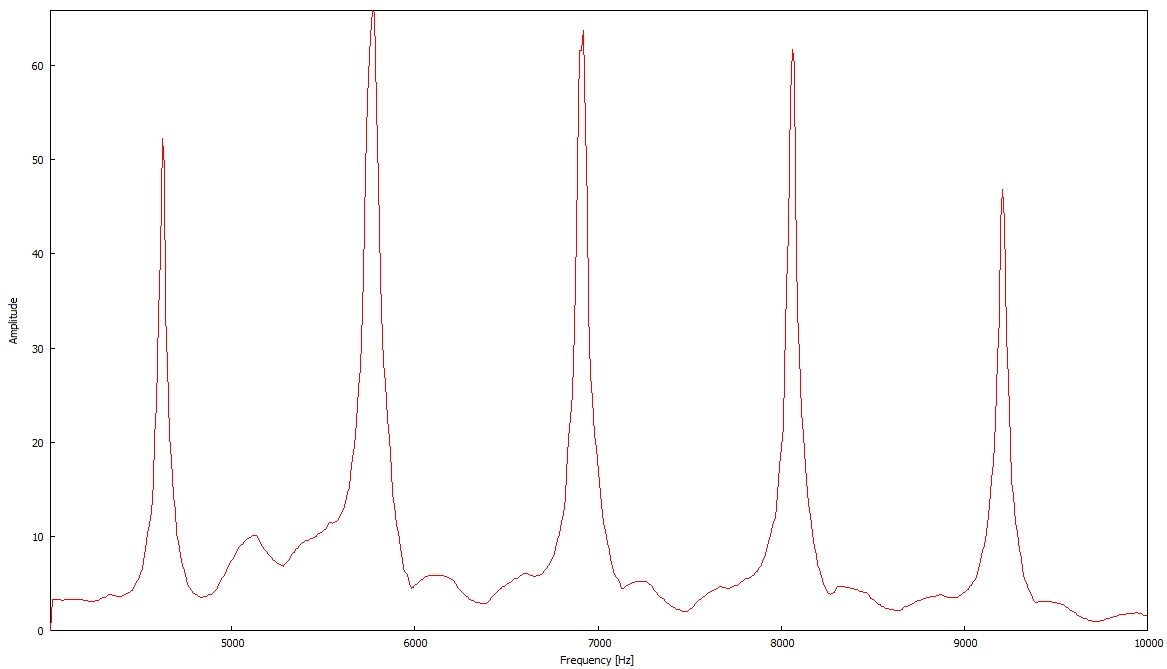
\includegraphics[width=1\textwidth]{content/messungen/Chapter4/4_1_150mm.jpg}
\caption{Spektrum eines 150~mm langen Rohres zwischen 4~kHz und 10~kHz.}
\label{fig:4_1_150}
\end{figure}

\begin{figure}
\centering
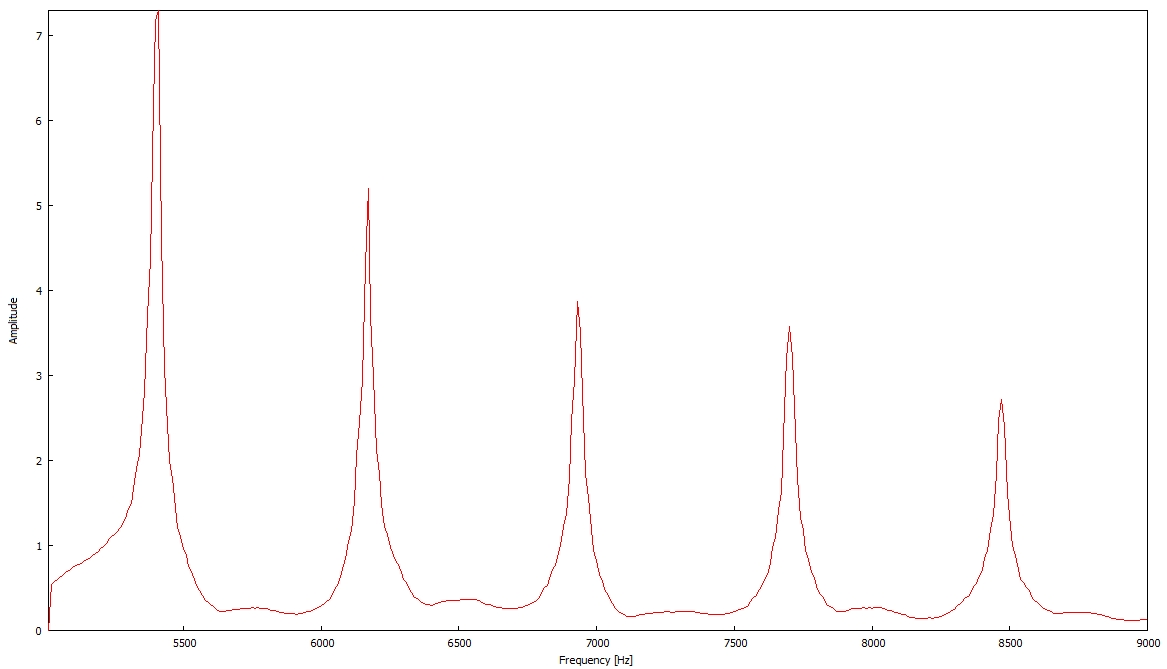
\includegraphics[width=1\textwidth]{content/messungen/Chapter4/4_1_225mm.jpg}
\caption{Spektrum eines 225~mm langen Rohres zwischen 5~kHz und 9~kHz.}
\label{fig:4_1_225}
\end{figure}

\begin{figure}
\centering
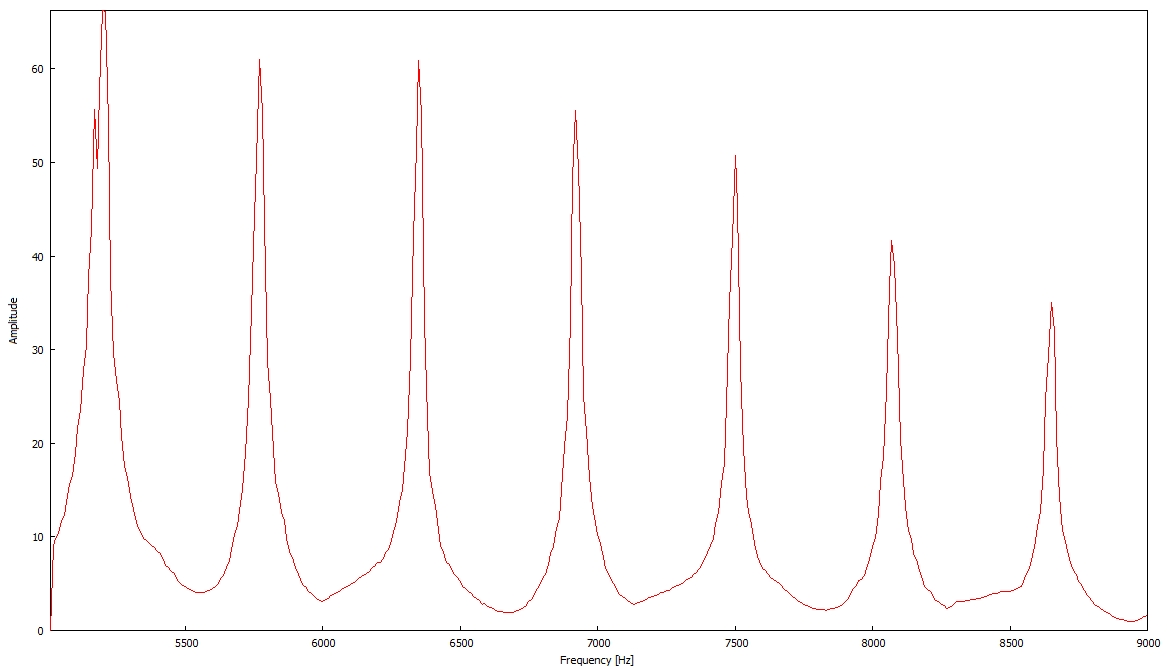
\includegraphics[width=1\textwidth]{content/messungen/Chapter4/4_1_300mm.jpg}
\caption{Spektrum eines 300~mm langen Rohres zwischen 5~kHz und 9~kHz.}
\label{fig:4_1_300}
\end{figure}

\begin{figure}
\centering
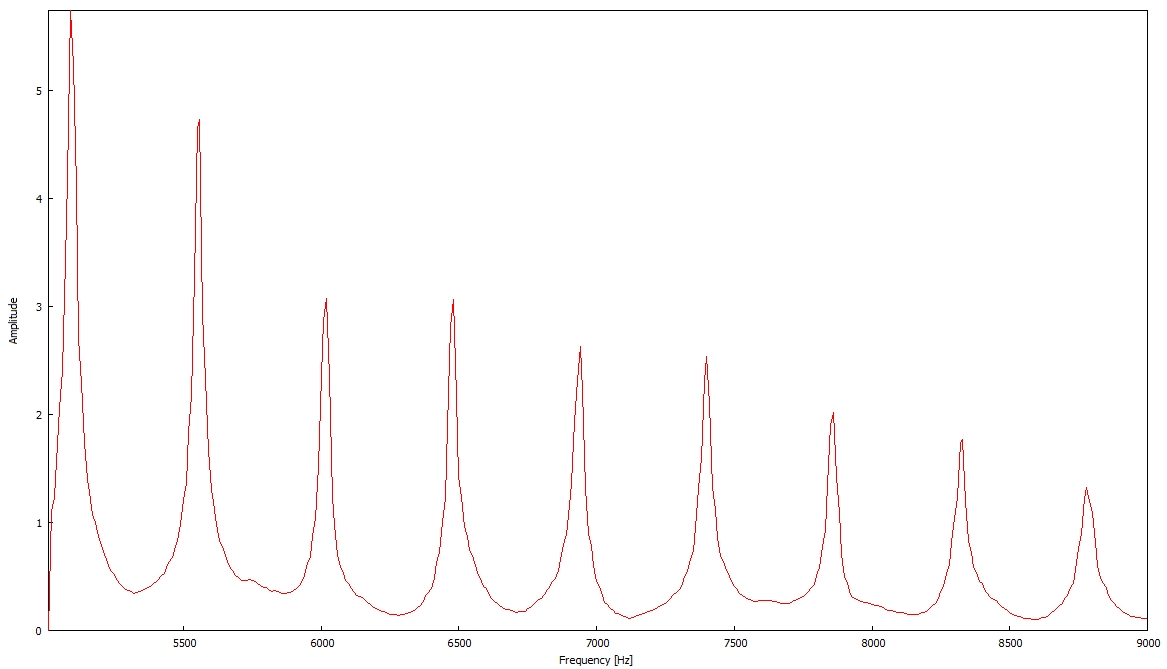
\includegraphics[width=1\textwidth]{content/messungen/Chapter4/4_1_375mm.jpg}
\caption{Spektrum eines 375~mm langen Rohres zwischen 5~kHz und 9~kHz.}
\label{fig:4_1_375}
\end{figure}

\begin{figure}
\centering
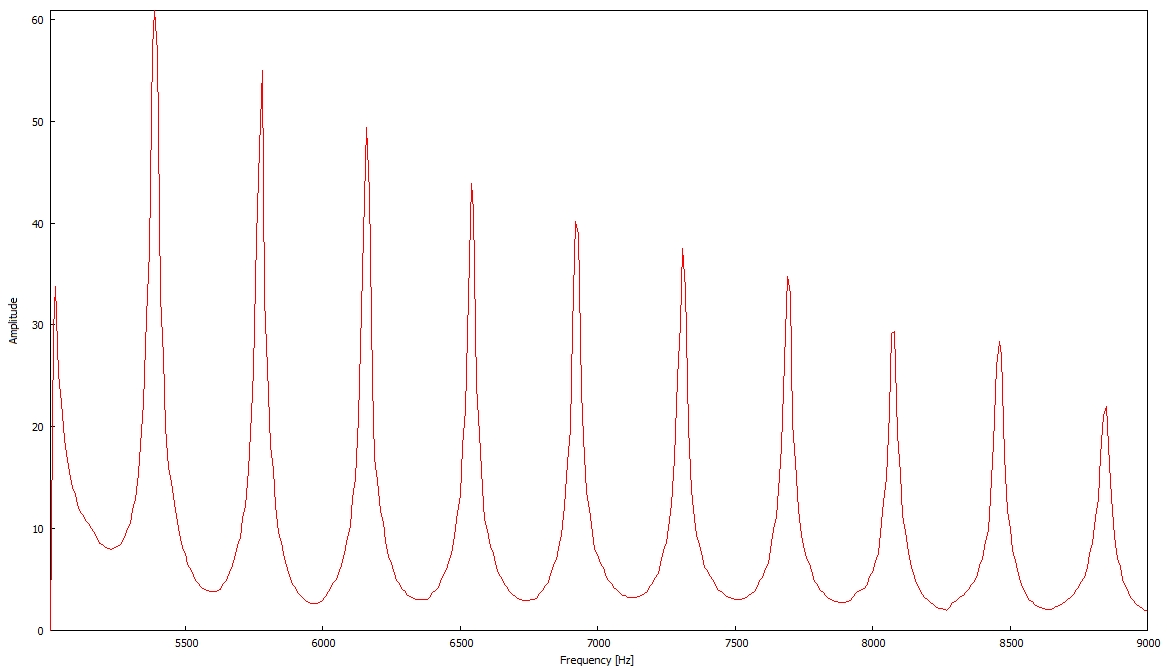
\includegraphics[width=1\textwidth]{content/messungen/Chapter4/4_1_450mm.jpg}
\caption{Spektrum eines 450~mm langen Rohres zwischen 5~kHz und 9~kHz.}
\label{fig:4_1_450}
\end{figure}

\begin{figure}
\centering
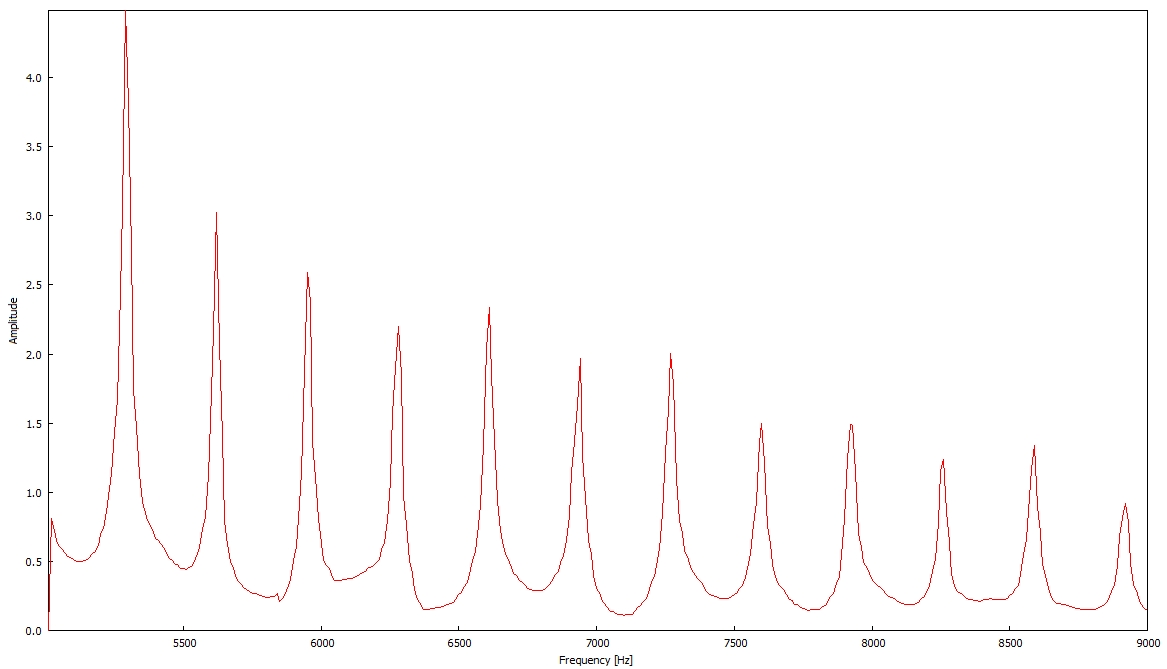
\includegraphics[width=1\textwidth]{content/messungen/Chapter4/4_1_525.jpg}
\caption{Spektrum eines 525~mm langen Rohres zwischen 5~kHz und 9~kHz.}
\label{fig:4_1_525}
\end{figure}

\begin{figure}
\centering
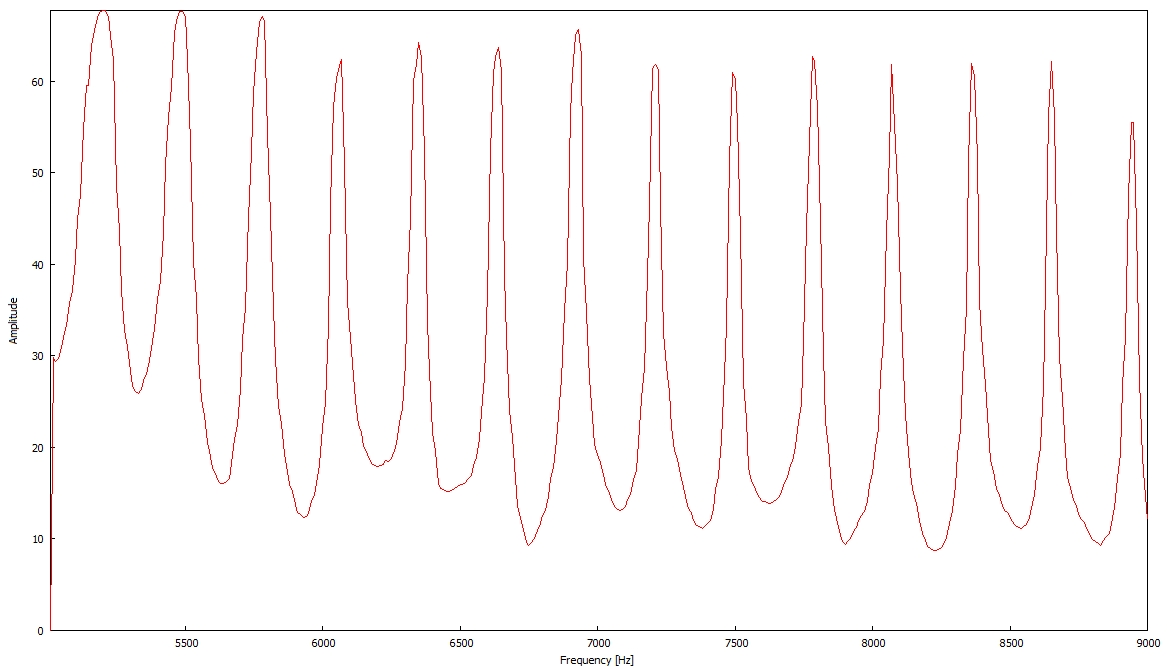
\includegraphics[width=1\textwidth]{content/messungen/Chapter4/4_1_600mm.jpg}
\caption{Spektrum eines 600~mm langen Rohres zwischen 5~kHz und 9~kHz.}
\label{fig:4_1_600}
\end{figure}
Die Peaks der Amplituden werden aus den Messdaten ausgelesen und werden in Tabelle \ref{tab:4:1} aufgeführt.
\begin{table}
\centering
\caption{Resonanzfrequenzen der verschiedenen Rohre im Frequenzbereich zwischen 5~kHz und 9~kHz, bzw. zwischen 4~kHz und 10~kHz für das Rohr der Länge 150~mm.}
\label{tab:4:1}
\begin{tabular}{c c c c c c c c c}
\hline
Rohrlänge  &600~mm&525~mm&450~mm&375~mm&300~mm& 225~mm& 150~mm & 75~mm \\ \hline
Resonanz- &5200& 5290& 5030 &5090 &5170 &5410 &4620 &6920\\
frequenzen&5480& 5620& 5390& 5560& 5770& 6170& 5770&\\
in Hz&5780& 5950& 5780& 6020& 6350& 6930& 6920&\\
&6070& 6280& 6160& 6480& 6920& 7700& 8060&\\
&6350& 6610& 6540& 6940& 7500& 8470& 9210&\\
&6640& 6940& 6920& 7400& 8070&& &\\
&6930& 7270& 7310& 7860& 8650&&&\\
&7210& 7600& 7690& 8330& &&&\\
&7490& 7920& 8080& 8780&&&&\\
&7780& 8260& 8460&&&&&\\
&8070& 8590&&&&&&\\
&8360& &&&&&&\\
&8650&&&&&&&\\
&8940&&&&&&&\\
\hline
\end{tabular}
\end{table}
Aus ihnen werden die Frequenzdifferenzen $\Delta f$ berechnet, um die Schallgeschwindigkeit zu bestimmen.
\begin{table}
\centering
\caption{Differenzen der Resonanzfrequenzen der verschiedenen Rohre im Frequenzbereich zwischen 5~kHz und 9~kHz, bzw. zwischen 4~kHz und 10~kHz für das Rohr der Länge 150~mm.}
\label{tab:4:2}
\begin{tabular}{c c c c c c c c c}
\hline
Rohrlänge  &600~mm&525~mm&450~mm&375~mm&300~mm& 225~mm& 150~mm & 75~mm \\ \hline
Differenz &280&330&360&470&600&760&1150&\\ 
der&300&330&390&460&580&760&1150&  \\ 
Resonanz-&290&330&380&460&570&770&1140&  \\ 
frequenzen&280&330&380&460&580&770&1150&  \\ 
in Hz&290&330&380&460&570&&&  \\ 
&290&330&390&460&580&  &  &  \\ 
&280&330&380&470&&  & &  \\ 
&280&320&390&450&  &  &  &  \\ 
&290&340&380&&  &  &  & \\ 
&290&330&&  &  &  &  &  \\ 
&290&&  &  &  &  &  &  \\ 
&290&  &  &  &  &  &  &  \\ 
&290&  &  &  &  &  &  & \\ 
\hline
Mittelwert&$287\pm 6$&$330\pm 4$&$381\pm 9$&$461\pm 6$&$580\pm 10$&$765\pm 5$&$1150\pm 4$ \\
in Hz &&&&&&&&\\
\hline
\end{tabular}
\end{table}
Mit 
\begin{align}
\Delta f=f_n-f_{n-1}=\frac{c}{\lambda_n}-\frac{c}{\lambda_{n-1}}=\frac{c}{2L}
\label{a:eq:1}
\end{align}
kann so aus den Mittelwerten der Frequenzdifferenzen aus Tabelle \ref{tab:4:2} die Schallgeschwindigkeit berechnet werden.
Es folgen die in Tabelle \ref{tab:4:3} aufgeführten Schallgeschwindigkeiten, deren Mittelwert 
\begin{align*}
c=(345\pm 2)~\text{ms}^{-1}
\end{align*}
das Ergebnis dieser Messung ist. Dabei wurde die Abweichung durch die Gauß'sche Fehlerfortpflanzung
\begin{align*}
\Delta c=\sqrt{\sum_{i=1}^n (\Delta c_i)^2}
\end{align*}
berechnet, wobei die $c_i$ die pro Rohr gemessenen Schallgeschwindigkeiten aus Tabelle \ref{tab:4:3} bezeichnen.
\begin{table}
\centering
\caption{Schallgeschwindigkeiten, berechnet nach Tabelle \ref{tab:4:2} und Gleichung (\ref{a:eq:1}).}
\label{tab:4:3}
\begin{tabular}{c c c c c c c c}
\hline
Rohrlänge in mm &600~mm&525~mm&450~mm&375~mm&300~mm& 225~mm& 150~mm \\ \hline
Schallgeschwindigkeit &$345\pm 7$&$347\pm 5$&$343\pm 8$&$346\pm 4$&$348\pm 6$&$344\pm 2$&$344\pm 1$\\
in ms$^{-1}$&&&&&&&\\
\hline
\end{tabular}
\end{table}
\FloatBarrier
Abbildung \ref{fig:4_2_1} zeigt ein Übersichtsspektrum eines 600~mm langen Rohres.
\begin{figure}
\centering
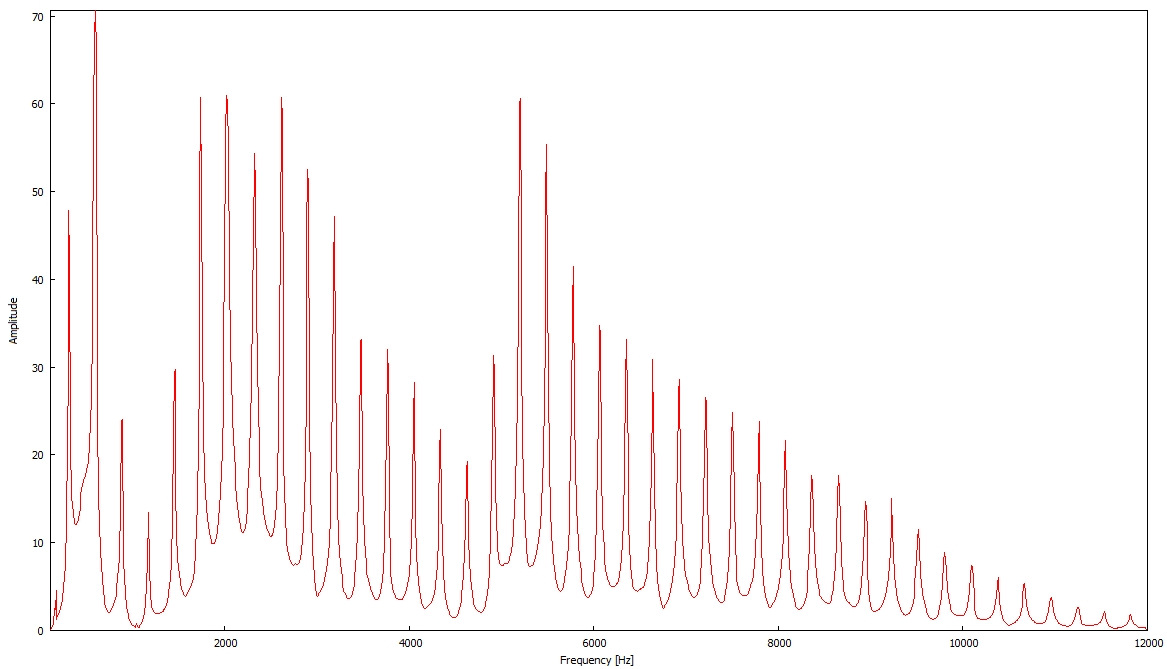
\includegraphics[width=1\textwidth]{content/messungen/Chapter4/4_2.jpg}
\caption{Resonanzspektrum eines Rohres der Länge 600~mm zwischen 0.1~kHz und 12~kHz.}
\label{fig:4_2_1}
\end{figure}
Durch abzählen der Peaks wird jedem Peak seine Wellenzahl
\begin{align}
k= n\frac{\pi}{L}
\end{align}
zugeordnet.
Abbildung \ref{fig:4_2_2} zeigt einen Plot der Resonanzfrequenzen gegen die entsprechenden Wellenzahlen.
\begin{figure}
\centering
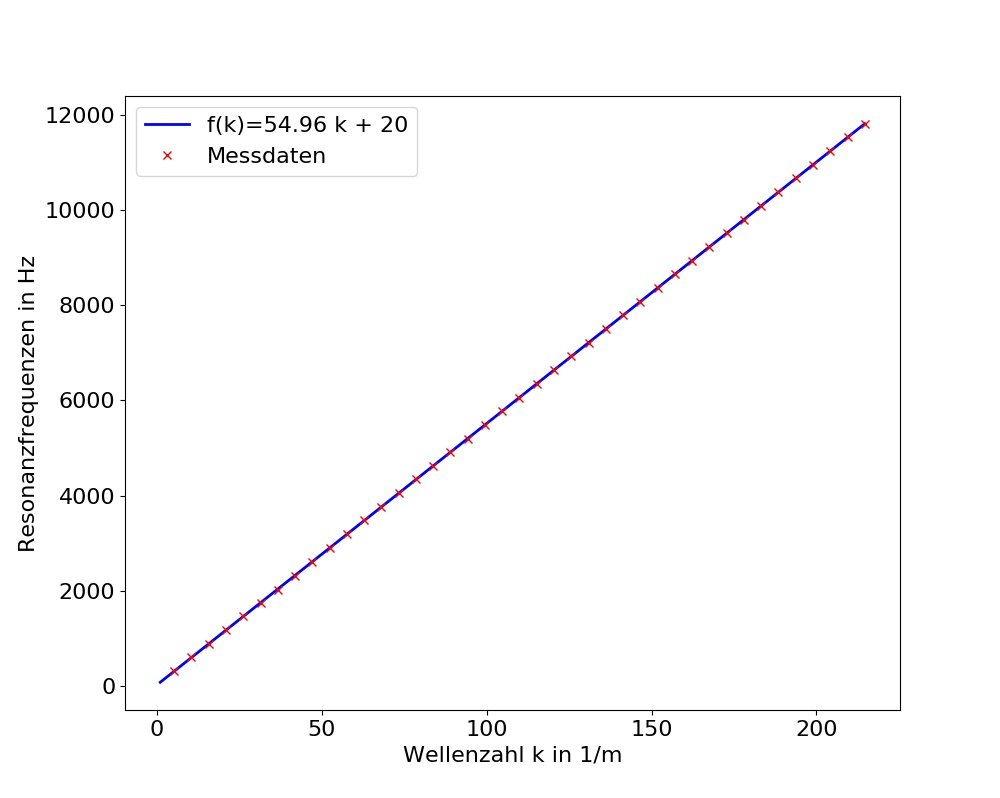
\includegraphics[width=\textwidth]{content/messungen/Chapter4/plot_4_2.jpg}
\caption{Resonanzfrequenzen in einem 600~mm Rohr in Abhängigkeit der Wellenzahl.}
\label{fig:4_2_2}
\end{figure}
Eine lineare Regression liefert die Ausgleichsgerade
\begin{align*}
f(k)=ak+b &&a=(54.96\pm 0.01)\text{ms}^{-1}&&b=(20\pm 1)\text{Hz} \text{ .}
\end{align*}
Es ist eindeutig eine lineare Dispersionsrelation zu erkennen.
Mit der bekannten Gleichung
\begin{align*}
f(k)=\frac{c}{2\pi}k
\end{align*}
lässt sich wiederholt die Schallgeschwindigkeit 
\begin{align*}
c=(345.33\pm0.06)\text{ms}^{-1}
\end{align*}
berechnen.
\FloatBarrier
Nun wird das 400~mm lange Rohr bestehend aus 8 Einheiten der Länge 50~mm und 6 Blenden mit den Durchmessern $d=10,13,16$~mm betrachtet.
Die Abbildungen \ref{fig:4_3_10} bis \ref{fig:4_3_16} zeigen die zugehörigen Resonanzspektren.
Für alle drei Blendendurchmesser stimmen die Wellenzahlen der Bänder überein, da die drei Anordnungen aus gleich vielen Einheitszellen bestehen.
Das erste Band liegen zwischen den Wellenzahlen $k^1_\text{min}=5.24~\text{m}^{-1}$ und $k^1_\text{max}=31.42~\text{m}^{-1}$, das zweite zwischen $k^2_\text{min}=36.65~\text{m}^{-1}$ und $k^2_\text{max}=62.83~\text{m}^{-1}$ und das dritte zwischen $k^3_\text{min}=68.07~\text{m}^{-1}$ und $k^3_\text{max}=94.25~\text{m}^{-1}$.
Die Resonanzstellen des vierten Bandes sind nicht alle klar erkennbar. 
Die Wellenzahlen dieses Bandes liegen zwischen $k^4_\text{min}=99.48~\text{m}^{-1}$ und $k^4_\text{max}=125.57~\text{m}^{-1}$.
Zwischen den Bändern ist jeweils eine Bandlücke.
An den Plots in der Brillouin Zone ist zu erkennen, dass die Steigung der Abhängigkeit $f(k)$ mit zunehmendem Blendendurchmesser größer wird.
Das hat zur folge, dass die Bandlücken kleiner werden.
\begin{figure}
\centering
\begin{subfigure}{0.65\textwidth}
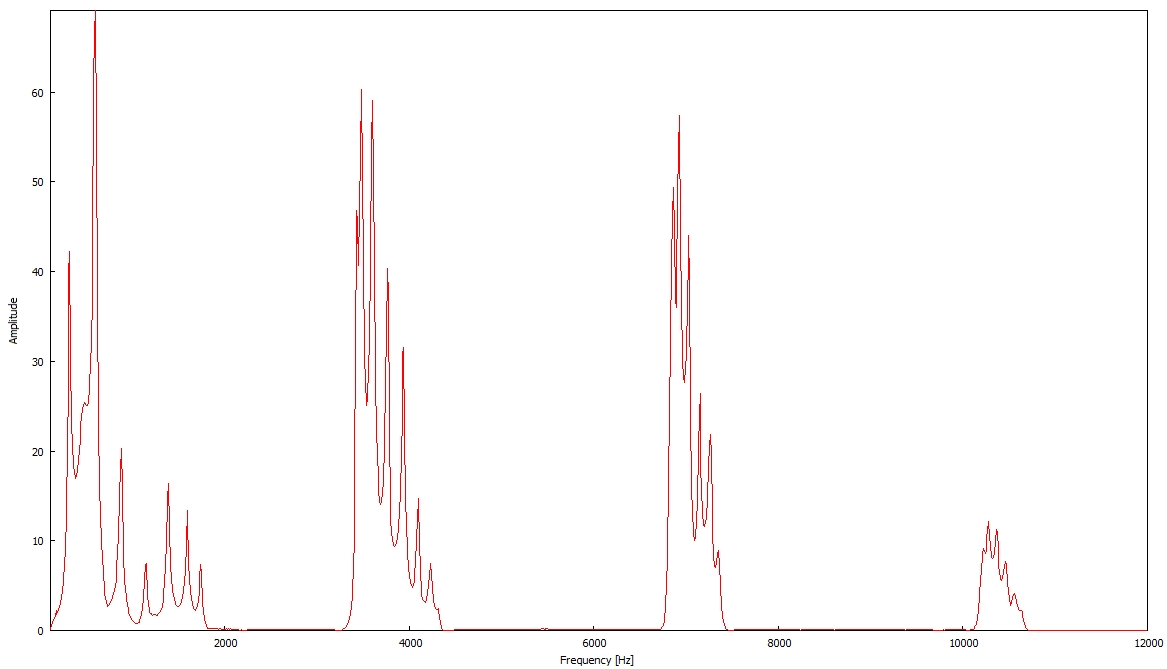
\includegraphics[width=\textwidth]{content/messungen/Chapter4/4_3_10mm.jpg}
\subcaption{Übliches Spektrum.}
\end{subfigure}
\begin{subfigure}{0.34\textwidth}
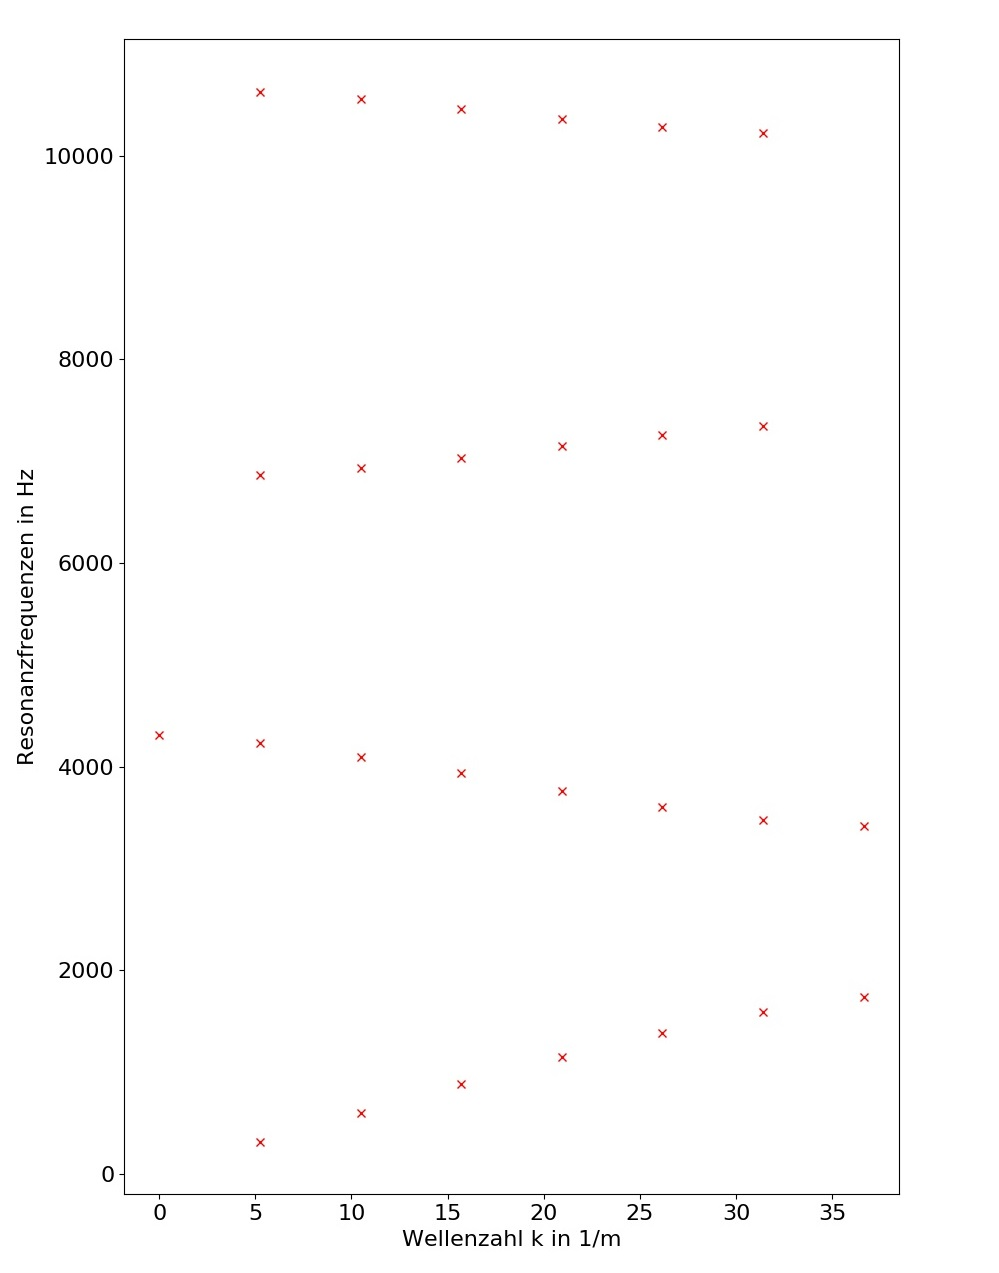
\includegraphics[width=\textwidth]{content/Scripts/4_3_10_red.jpg}
\subcaption{Resonanzfrequenzen in Abhängigkeit von der Wellenzahl in der Brillouin Zone.}
\end{subfigure}
\caption{Resonanzspektrum eines 400~mm langen Rohres mit 7 10~mm Blenden, jeweils im Abstand von 50~mm, zwischen 0.1~kHz und 12~kHz.}
\label{fig:4_3_10}
\end{figure}
\begin{figure}
\centering
\begin{subfigure}{0.65\textwidth}
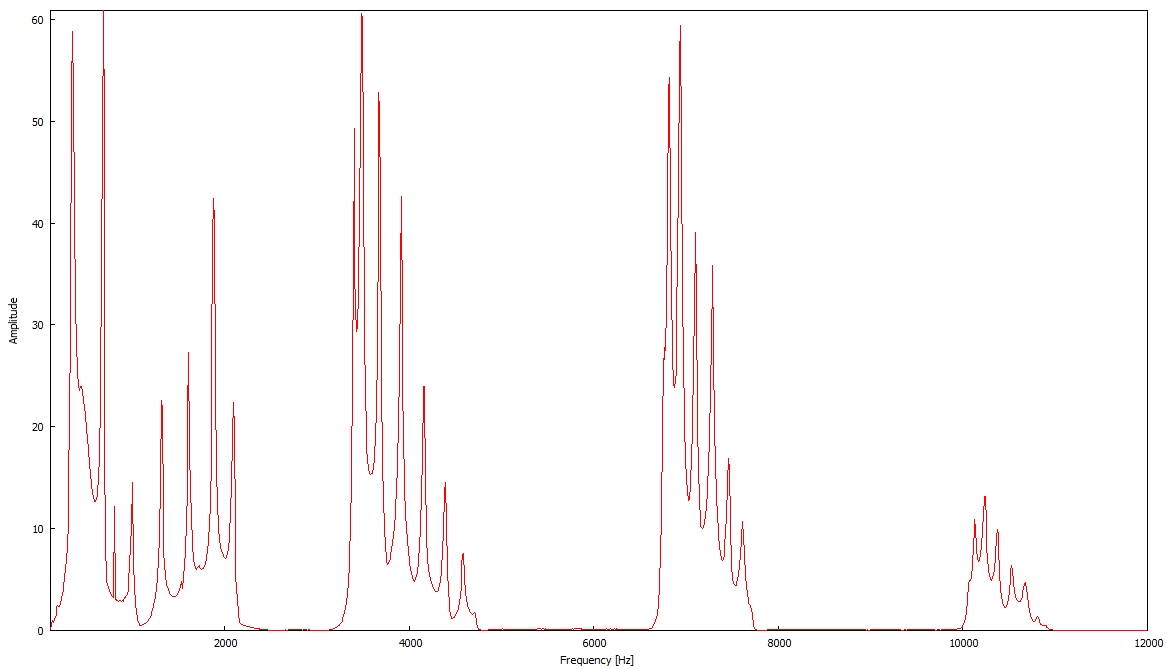
\includegraphics[width=\textwidth]{content/messungen/Chapter4/4_3_13mm.jpg}
\subcaption{Übliches Spektrum.}
\end{subfigure}
\begin{subfigure}{0.34\textwidth}
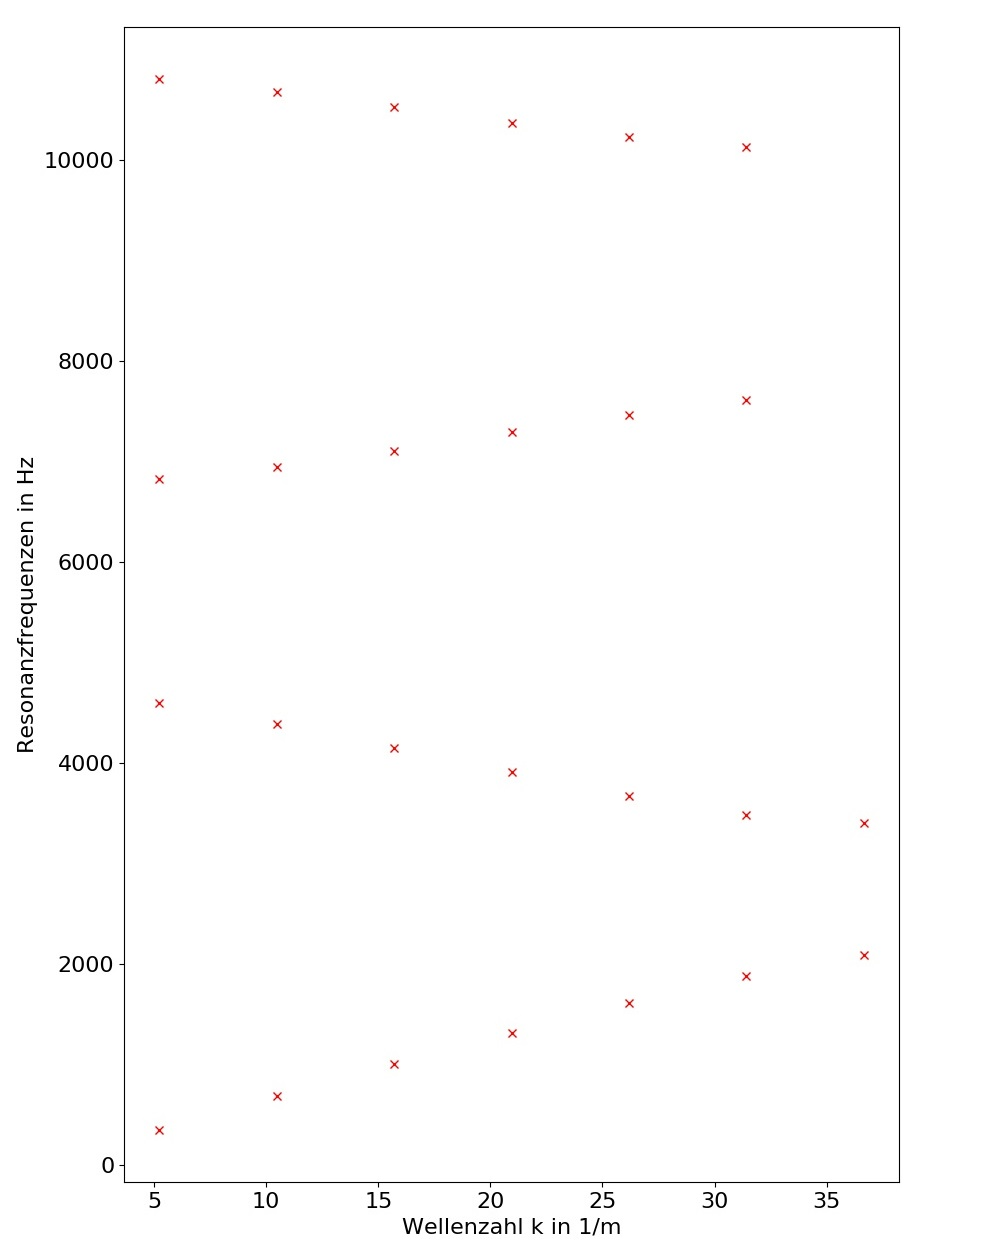
\includegraphics[width=\textwidth]{content/Scripts/4_3_13_red.jpg}
\subcaption{Resonanzfrequenzen in Abhängigkeit von der Wellenzahl in der Brillouin Zone.}
\end{subfigure}
\caption{Resonanzspektrum eines 400~mm langen Rohres mit 7 13~mm Blenden, jeweils im Abstand von 50~mm, zwischen 0.1~kHz und 12~kHz.}
\label{fig:4_3_13}
\end{figure}
\begin{figure}
\centering
\begin{subfigure}{0.65\textwidth}
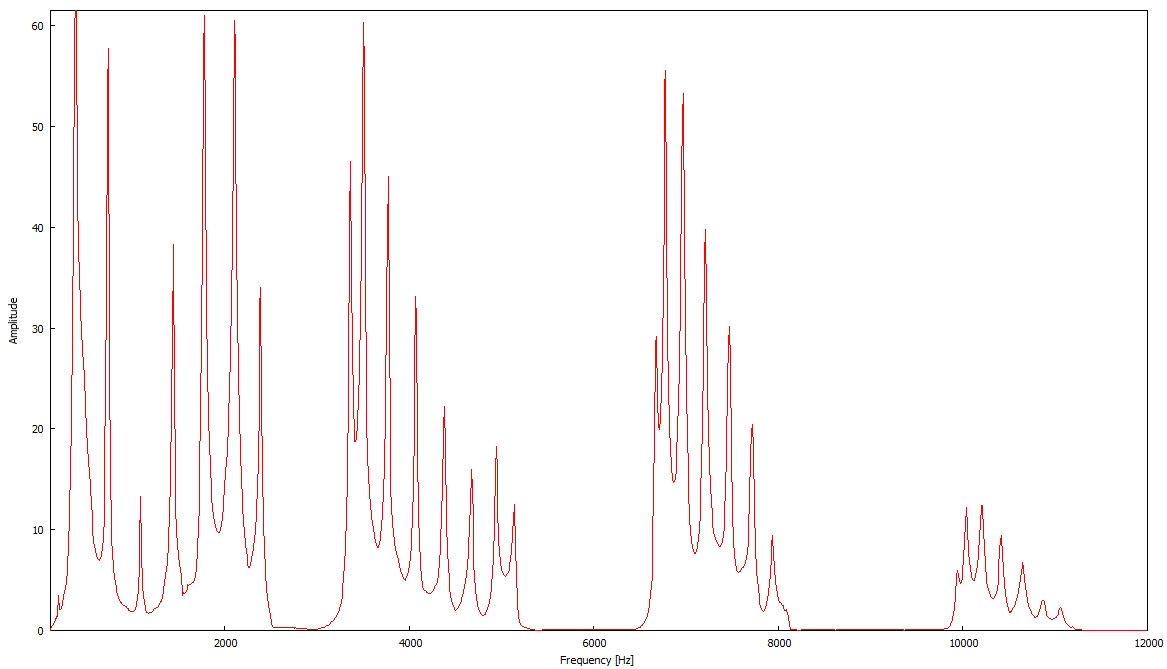
\includegraphics[width=\textwidth]{content/messungen/Chapter4/4_3_16mm.jpg}
\subcaption{Übliches Spektrum.}
\end{subfigure}
\begin{subfigure}{0.34\textwidth}
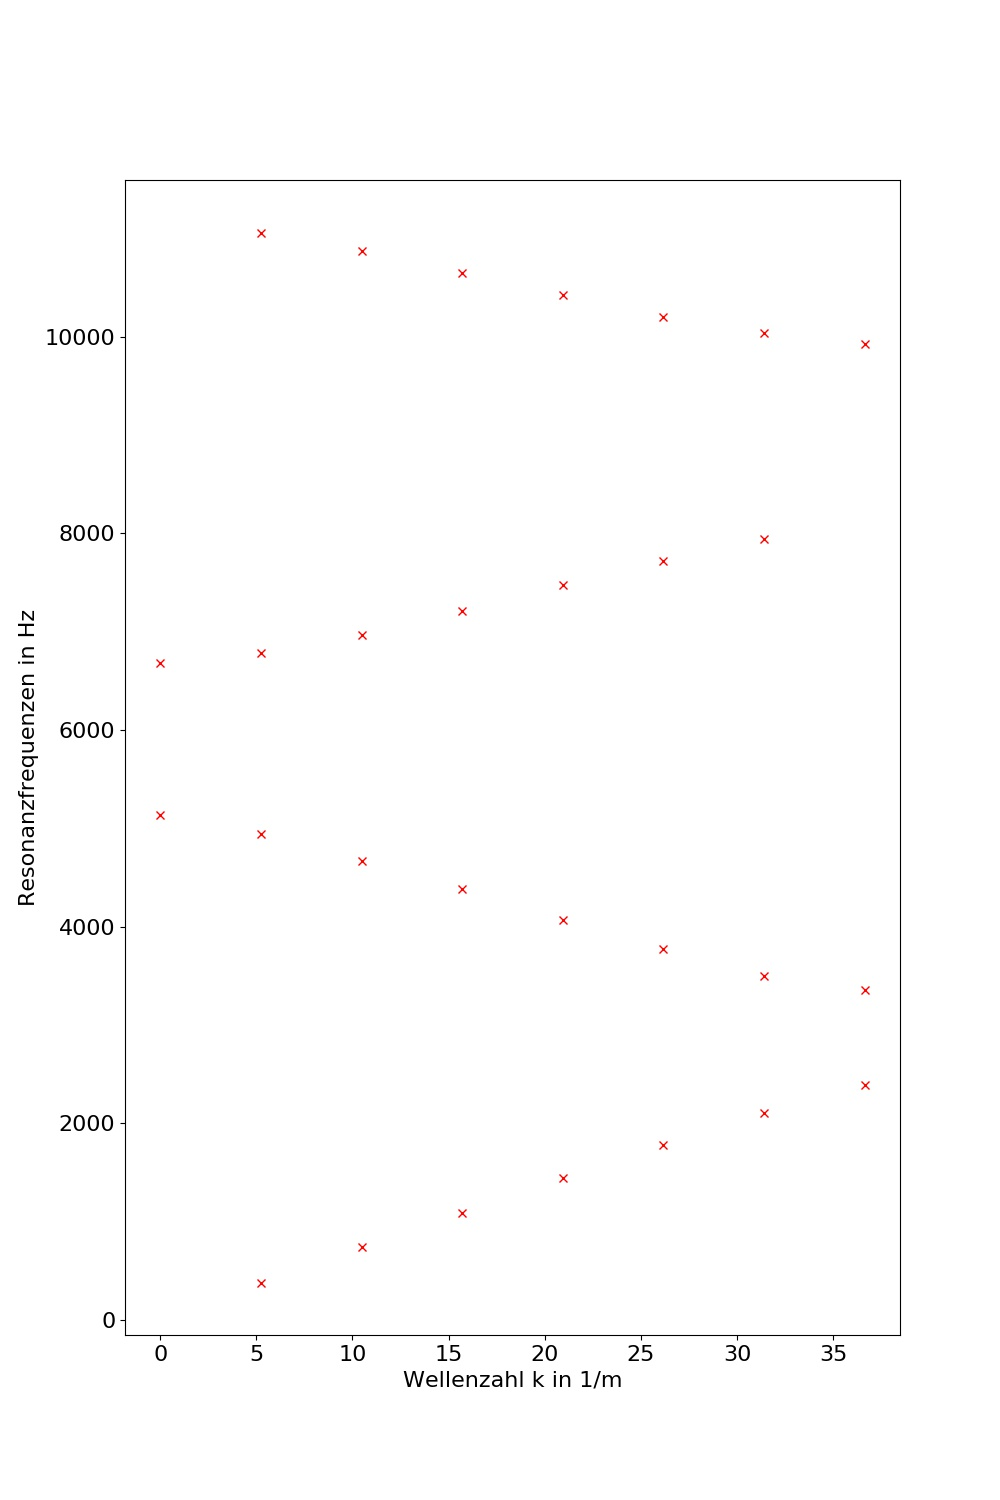
\includegraphics[width=\textwidth]{content/Scripts/4_3_16_red.jpg}
\subcaption{Resonanzfrequenzen in Abhängigkeit von der Wellenzahl in der Brillouin Zone.}
\end{subfigure}
\caption{Resonanzspektrum eines 400~mm langen Rohres mit 7 16~mm Blenden, jeweils im Abstand von 50~mm, zwischen 0.1~kHz und 12~kHz.}
\label{fig:4_3_16}
\end{figure}

Im Vergleich zu Abbildung \ref{fig:4_3_16} zeigen Abbildung \ref{fig:4_4_10} bzw. \ref{fig:4_4_12} jeweils 10 bzw. 12 50~mm Rohre, die durch 16~mm Blenden getrennt sind.
\begin{figure}
\centering
\begin{subfigure}{0.65\textwidth}
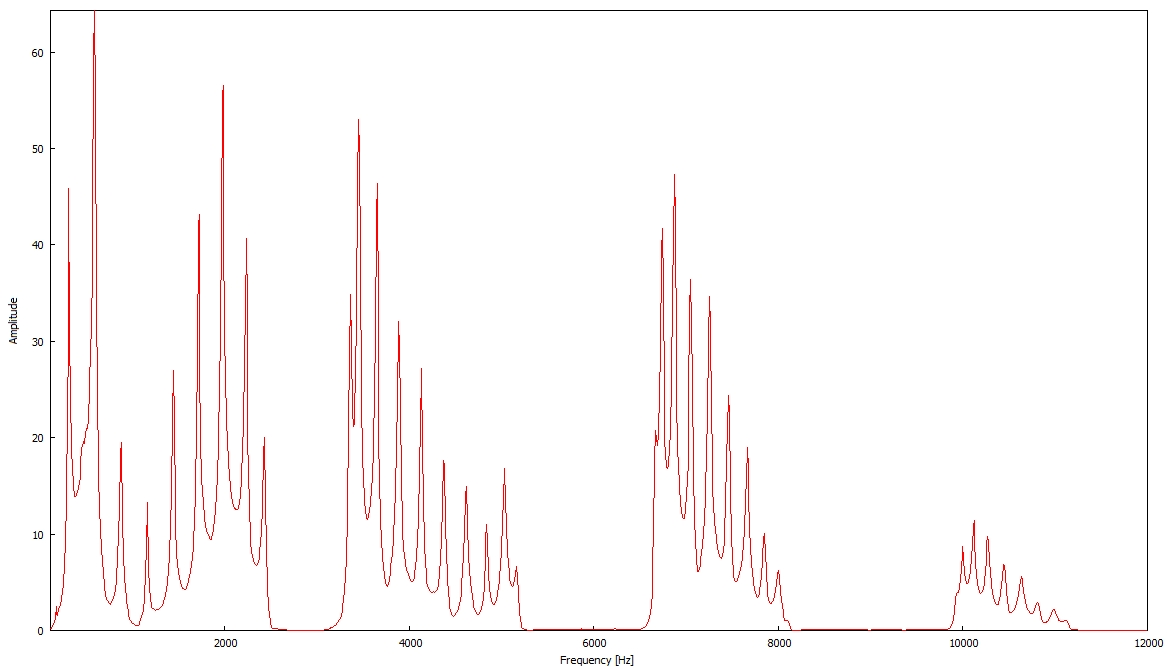
\includegraphics[width=\textwidth]{content/messungen/Chapter4/4_4_10x50.jpg}
\subcaption{Übliches Spektrum.}
\end{subfigure}
\begin{subfigure}{0.34\textwidth}
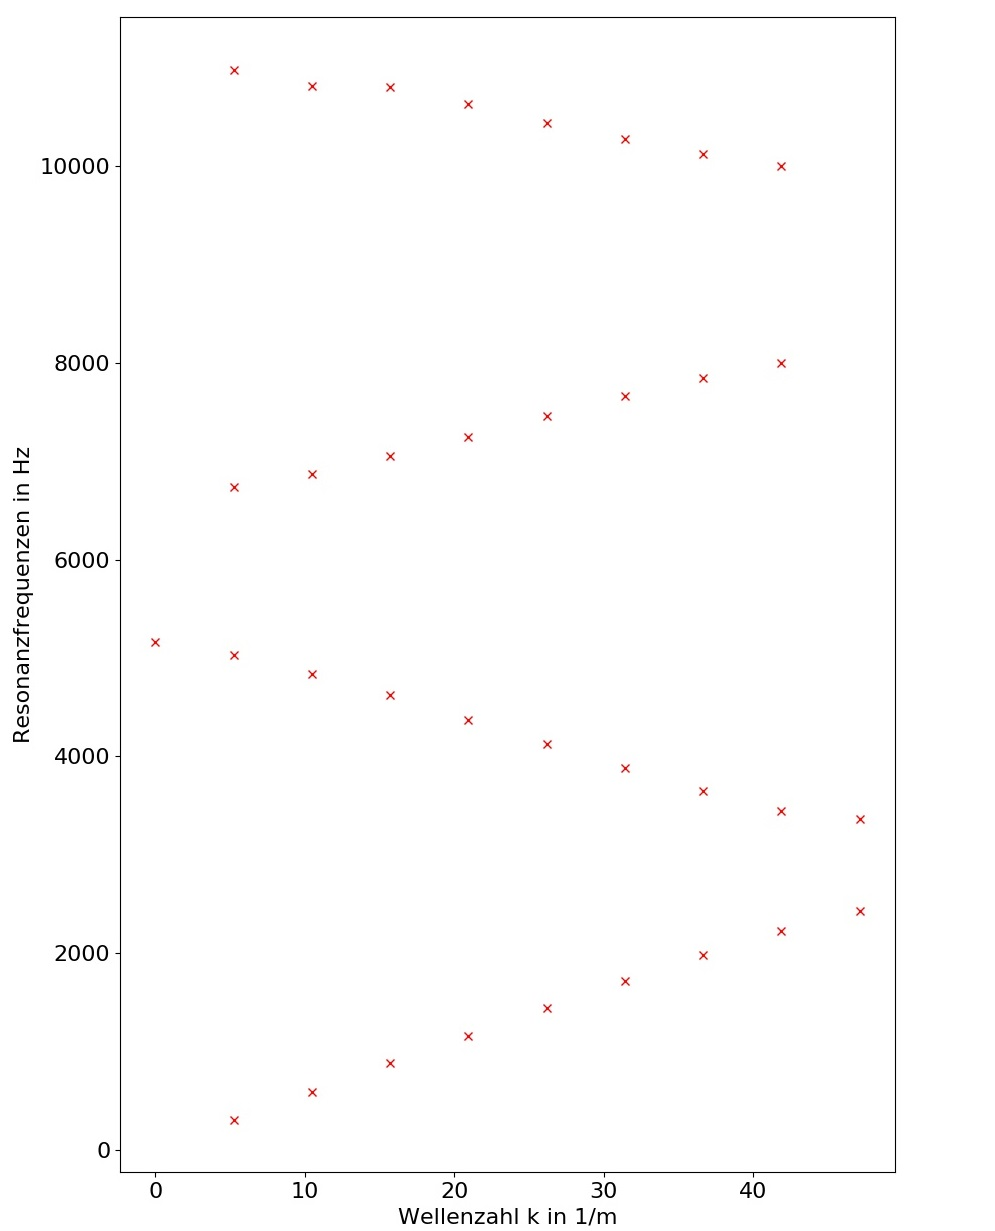
\includegraphics[width=\textwidth]{content/Scripts/4_4_10_red.jpg}
\subcaption{Resonanzfrequenzen in Abhängigkeit von der Wellenzahl in der Brillouin Zone.}
\end{subfigure}
\caption{Resonanzspektrum eines 500~mm langen Rohres mit 9 16~mm Blenden, jeweils im Abstand von 50~mm, zwischen 0.1~kHz und 12~kHz.}
\label{fig:4_4_10}
\end{figure}
\begin{figure}
\centering
\begin{subfigure}{0.65\textwidth}
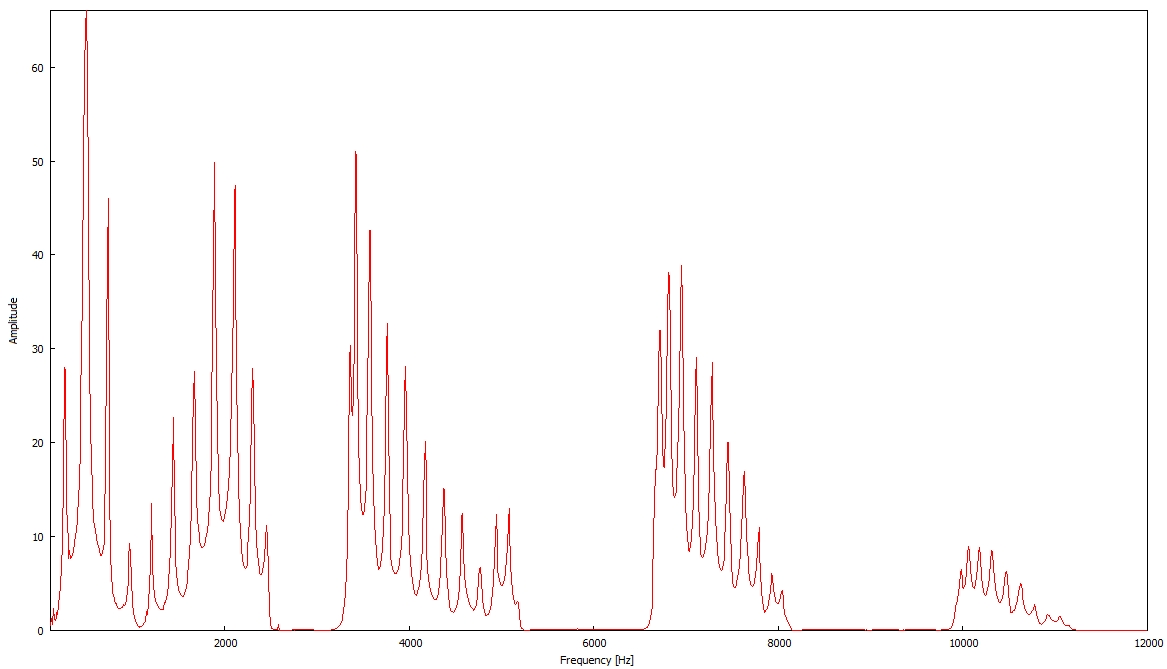
\includegraphics[width=\textwidth]{content/messungen/Chapter4/4_4_12x50.jpg}
\subcaption{Übliches Spektrum.}
\end{subfigure}
\begin{subfigure}{0.34\textwidth}
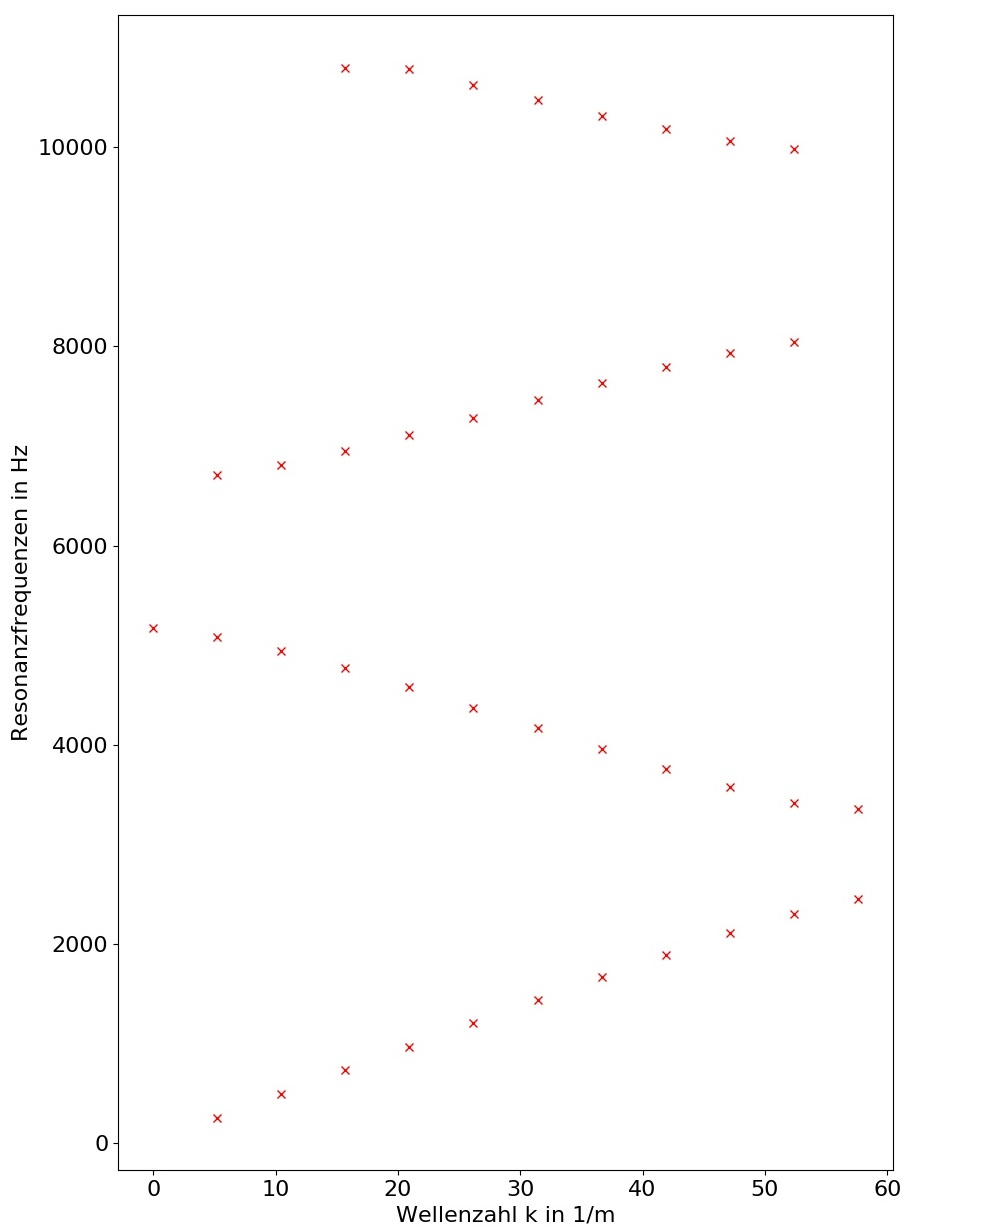
\includegraphics[width=\textwidth]{content/Scripts/4_4_12_red.jpg}
\subcaption{Resonanzfrequenzen in Abhängigkeit von der Wellenzahl in der Brillouin Zone.}
\end{subfigure}
\caption{Resonanzspektrum eines 600~mm langen Rohres mit 11 16~mm Blenden, jeweils im Abstand von 50~mm, zwischen 0.1~kHz und 12~kHz.}
\label{fig:4_4_12}
\end{figure}
Die Abbildungen zeigen, dass die Bandlücken sich mit steigender Anzahl der Einheitszellen nicht verändern. 
Auch die Dispersionsrelation bleibt gleich.
Werden 75~mm Rohre anstelle der 50~mm Rohre verwendet, flacht die gesamte Dispersion ab, die Bänder rücken dichter aneinander heran (vgl. Abbildung \ref{fig:4_5}).
\begin{figure}
\centering
\begin{subfigure}{0.65\textwidth}
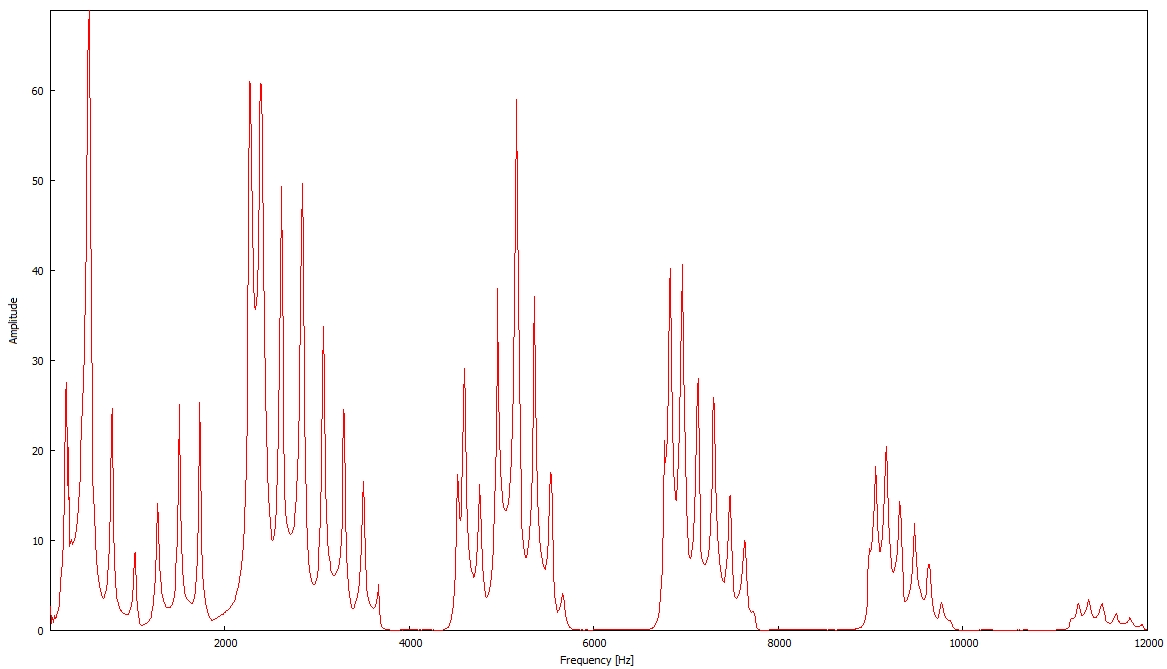
\includegraphics[width=\textwidth]{content/messungen/Chapter4/4_5.jpg}
\subcaption{Übliches Spektrum.}
\end{subfigure}
\begin{subfigure}{0.34\textwidth}
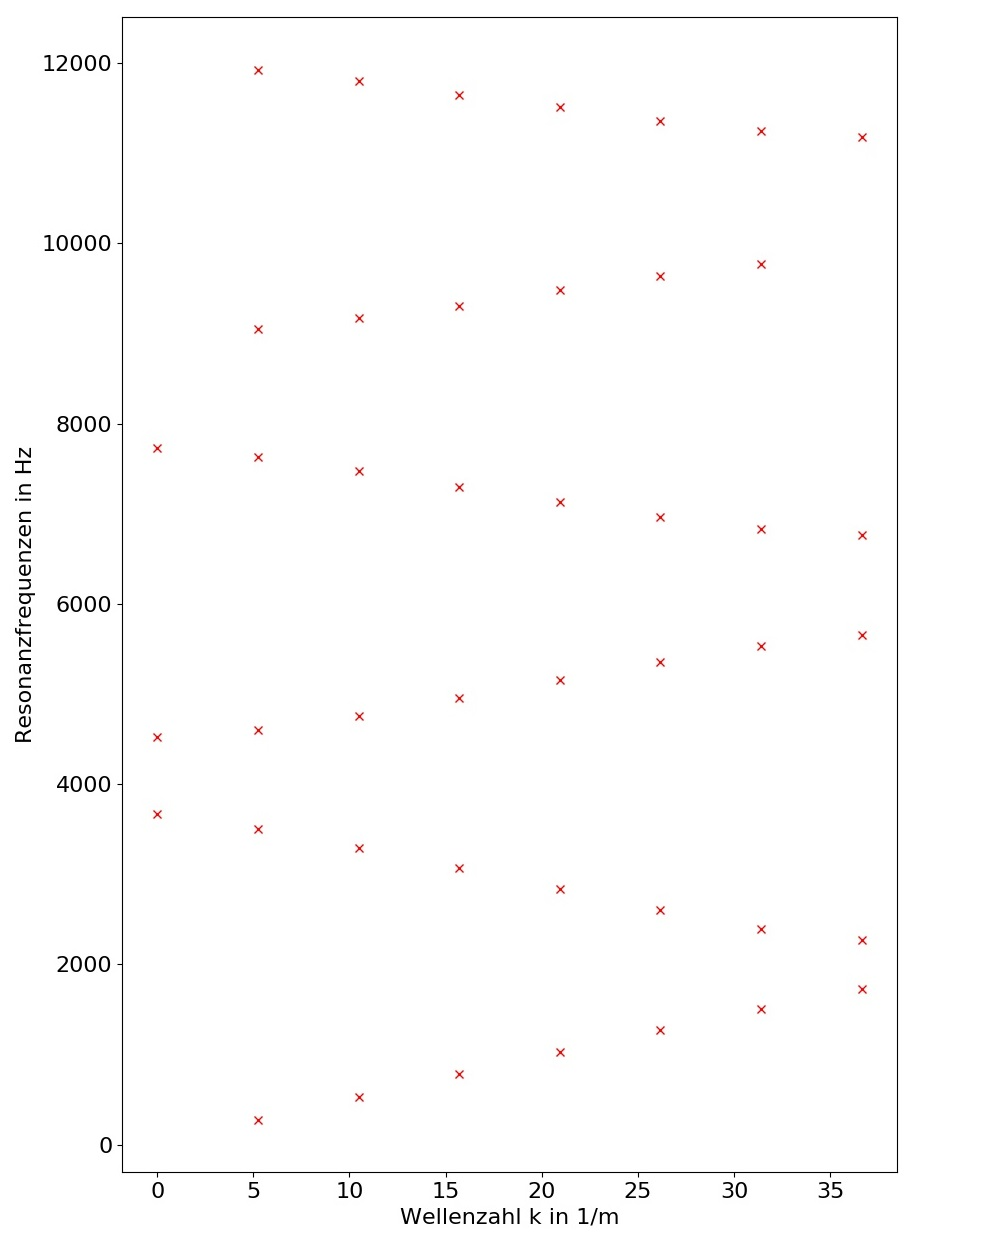
\includegraphics[width=\textwidth]{content/Scripts/4_5_red.jpg}
\subcaption{Resonanzfrequenzen in Abhängigkeit von der Wellenzahl in der Brillouin Zone.}
\end{subfigure}
\caption{Resonanzspektrum eines 600~mm langen Rohres mit 7 16~mm Blenden, jeweils im Abstand von 75~mm, zwischen 0.1~kHz und 12~kHz.}
\label{fig:4_5}
\end{figure}

Zuletzt wird für das 400~mm Rohr mit 7 Blenden des Durchmessers 16~mm die Dichte 
\begin{align*}
\rho(f)=\frac{1}{f_{i+1}-f_i}
\end{align*}
der Energieniveaus bestimmt.
Wie an Abbildung \ref{fig:dos} zu erkennen ist, ist die Dichte am Energetisch höheren Rand jedes Bandes wesentlich höher als im restlichen Band.
\begin{figure}
\centering
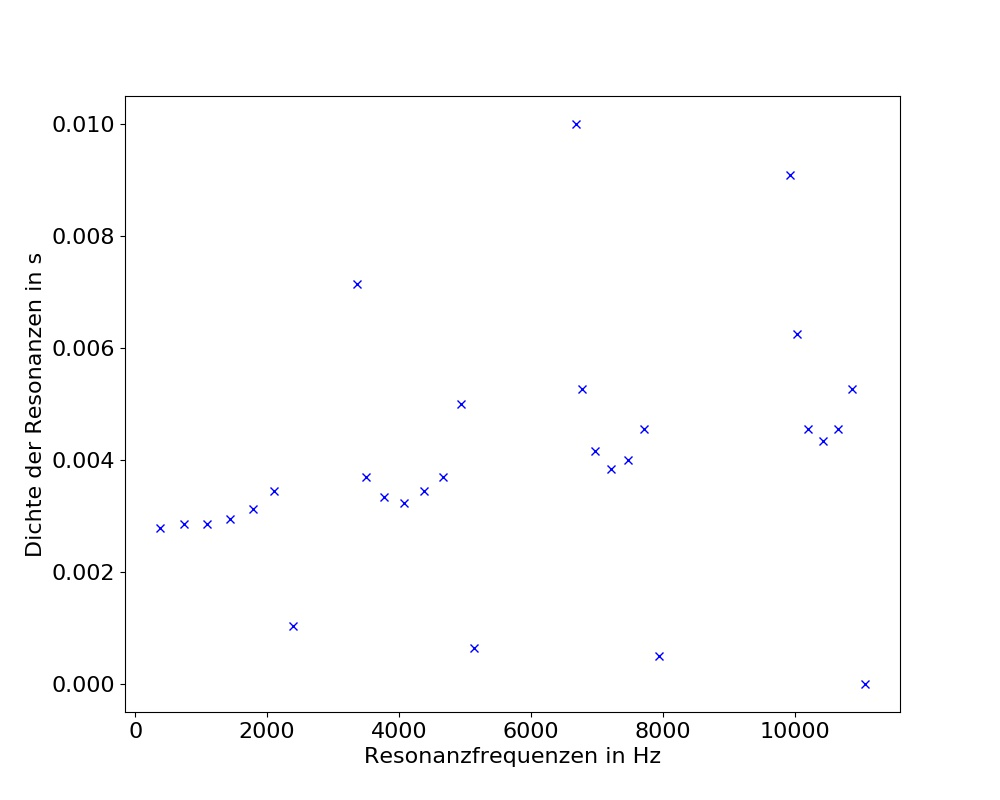
\includegraphics[width=\textwidth]{content/Scripts/dos.jpg}
\caption{Zustandsdichten in Abhängigkeit von der Frequenz.}
\label{fig:dos}
\end{figure}
\FloatBarrier
\subsection{Atom Molekül Ketten}
\label{subsec:Atom Molekül Ketten}
Das Spektrum eines 50~mm langes Rohres wird in Abbildung \ref{fig:4b_1} dargestellt.
\begin{figure}
\centering
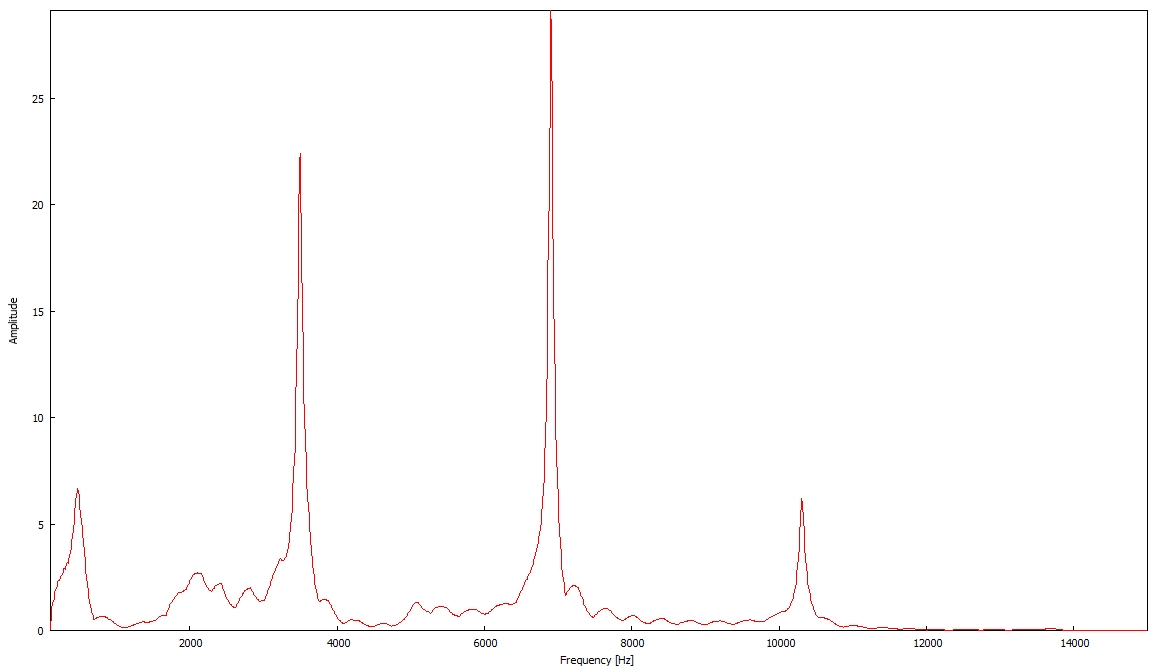
\includegraphics[width=\textwidth]{content/messungen/Chapter4b/4b_1.jpg}
\caption{Spektrum eines 50~mm langen Rohres zwischen 0.1~kHz und 15~kHz. Der Peak bei 0.48~kHz ist durch die Bauart der Soundkarte bedingt und ist daher keine Resonanzstelle.}
\label{fig:4b_1}
\end{figure}
Wie an dieser Abbildung zu sehen ist geht das Signal an der verwendeten Soundkarte ab 14~kHz gegen Null, sodass eine Vermessung des Spektrums oberhalb von 14~kHz nicht möglich ist. 
Da transversale Wellen erst ab ca. 16~kHz beobachtet werden können, können nur über longitudinale Wellen Aussagen getroffen werden.
Letztere sind hier ohnehin von alleinigem Interesse.
Im Vergleich dazu zeigt Abbildung \ref{fig:4b_2} das Spektrum eines 75~mm langen Rohres im gleichen Frequenzbereich.
\begin{figure}
\centering
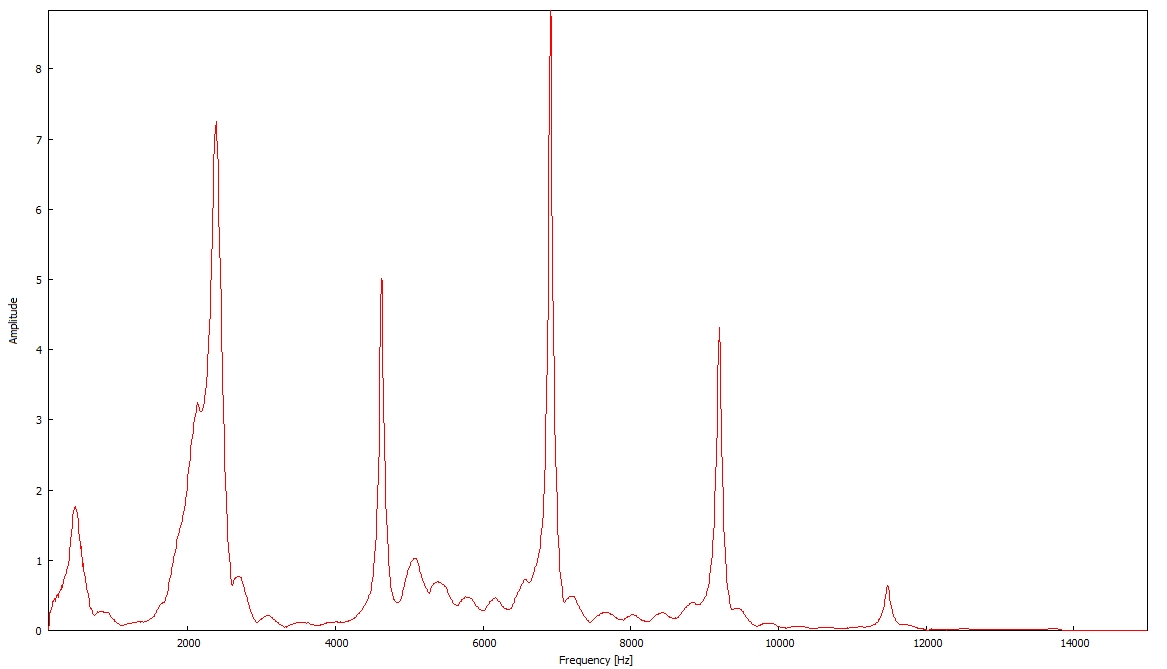
\includegraphics[width=\textwidth]{content/messungen/Chapter4b/4b_2.jpg}
\caption{Spektrum eines 75~mm langen Rohres zwischen 0.1~kHz und 15~kHz. Der Peak bei 0.48~kHz ist durch die Bauart der Soundkarte bedingt und ist daher keine Resonanzstelle.}
\label{fig:4b_2}
\end{figure}
Es wird klar, dass sich die Resonanzstellen zu niedrigeren Energien hin verschieben und etwas dichter werden.

\noindent Die Abbildungen \ref{fig:4b_3_10}, \ref{fig:4b_3_13} und \ref{fig:4b_3_16}  zeigen die Spektren von zwei durch eine Blende des Durchmessers $d=10,13,16$~mm getrennten 50~mm Rohren.
\begin{figure}
\centering
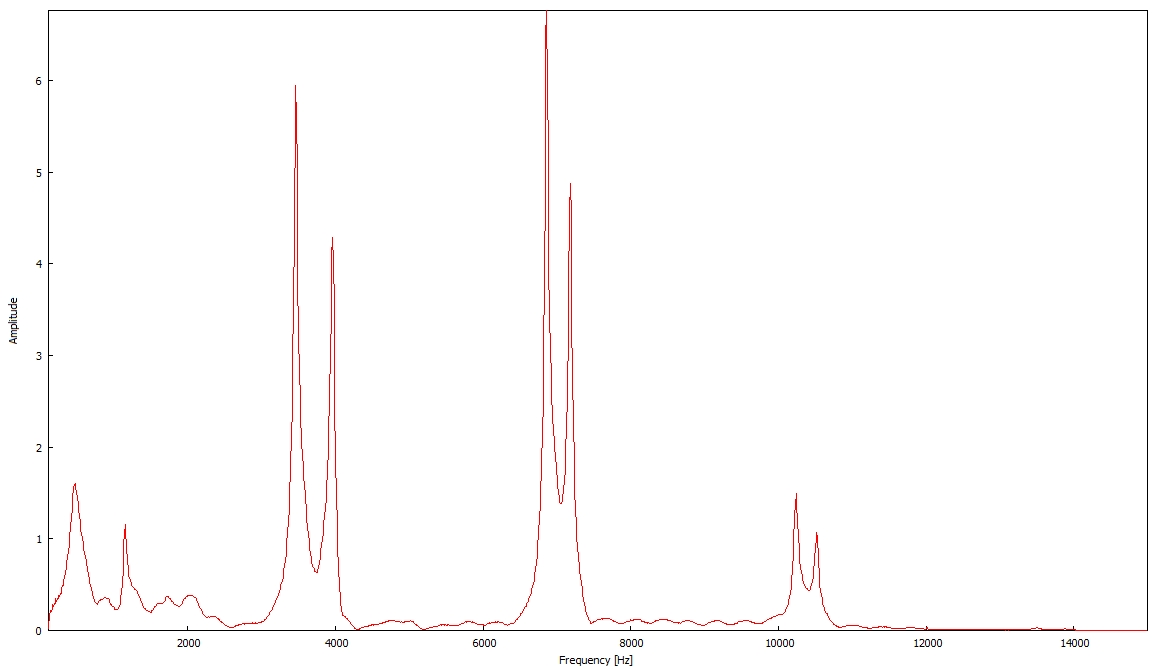
\includegraphics[width=\textwidth]{content/messungen/Chapter4b/4b_3_10.jpg}
\caption{Spektrum zwischen 0.1~kHz und 15~kHz zweier 50~mm langen Rohre, die durch eine Blende vom Durchmesser 10~mm getrennt sind. Dabei ist je Band der Zustand mit der geringsten Frequenz der Bindende Zustand. Der erste Peak ist durch die Wechselwirkung von Mikrophon und Lautsprecher bedingt und ist daher keine Resonanzstelle.}
\label{fig:4b_3_10}
\end{figure}
\begin{figure}
\centering
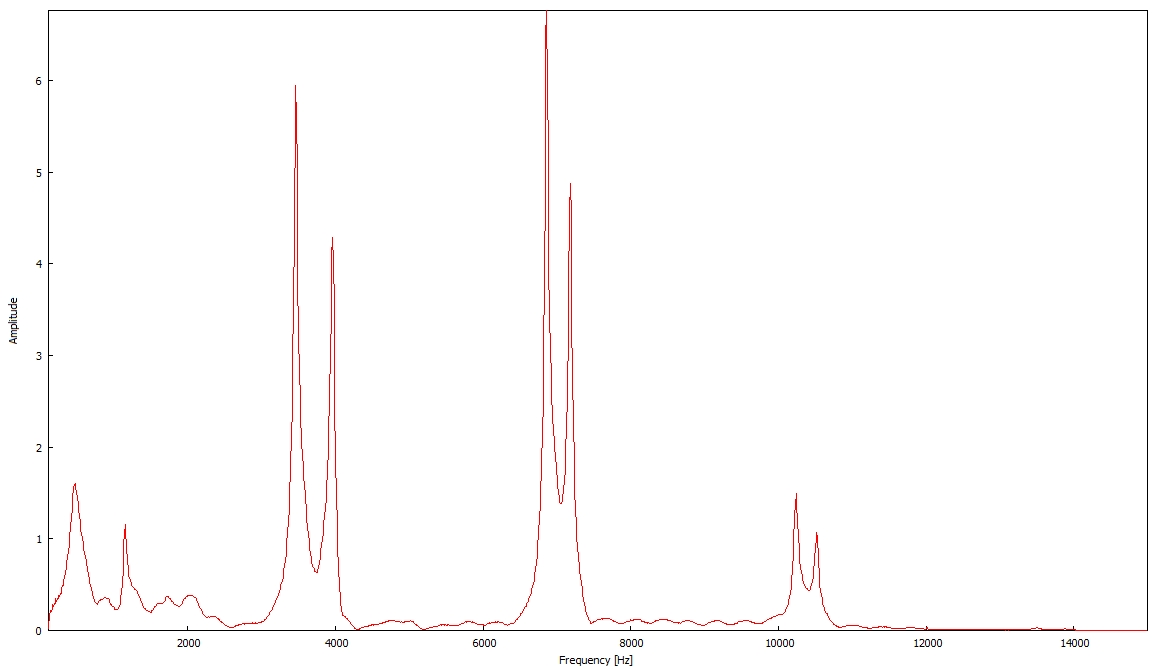
\includegraphics[width=\textwidth]{content/messungen/Chapter4b/4b_3_10.jpg}
\caption{Spektrum zwischen 0.1~kHz und 15~kHz zweier 50~mm langen Rohre, die durch eine Blende vom Durchmesser 13~mm getrennt sind. Dabei ist je Band der Zustand mit der geringsten Frequenz der Bindende Zustand. Der erste Peak ist durch die Wechselwirkung von Mikrophon und Lautsprecher bedingt und ist daher keine Resonanzstelle.}
\label{fig:4b_3_13}
\end{figure}
\begin{figure}
\centering
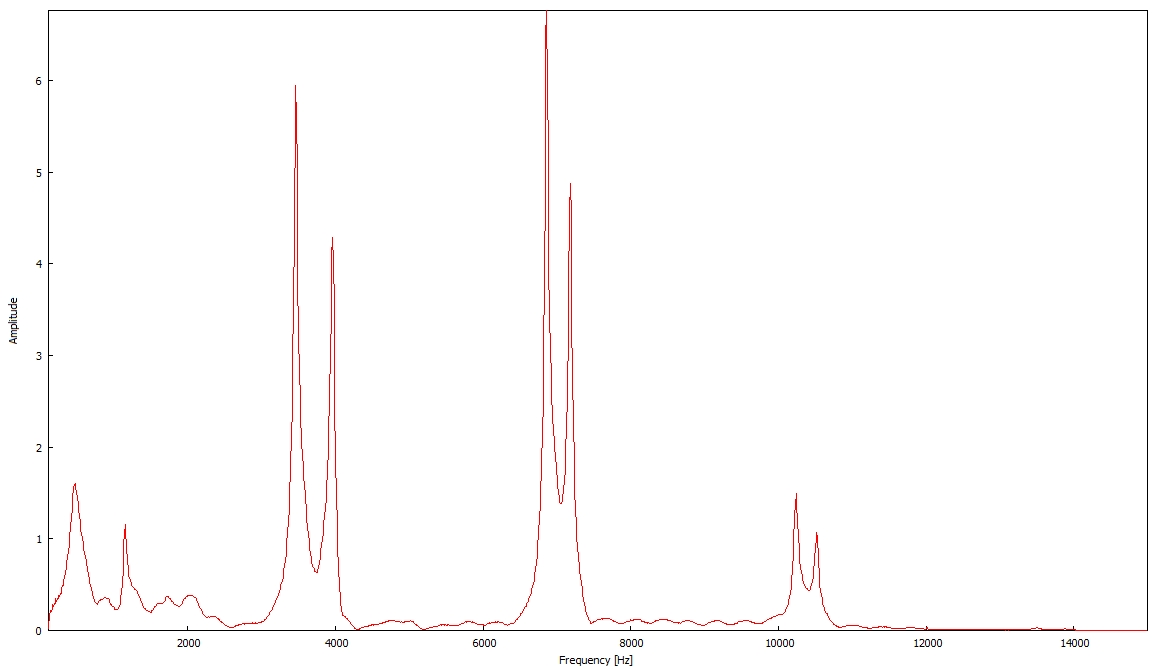
\includegraphics[width=\textwidth]{content/messungen/Chapter4b/4b_3_10.jpg}
\caption{Spektrum zwischen 0.1~kHz und 15~kHz zweier 50~mm langen Rohre, die durch eine Blende vom Durchmesser 16~mm getrennt sind. Dabei ist je Band der Zustand mit der geringsten Frequenz der Bindende Zustand. Der erste Peak ist durch die Wechselwirkung von Mikrophon und Lautsprecher bedingt und ist daher keine Resonanzstelle.}
\label{fig:4b_3_16}
\end{figure}
Durch das hinzufügen der Blende splitten sich die Energieniveaus in Bänder.
Der Durchmesser der Blende beeinflusst wie weit zwei Peaks des gleichen Bandes auseinander liegen.
Anstelle von 2 50~mm Rohren werden nun mehrere hintereinander geschaltet.
Die Spektren für 3 Rohre mit jeweils verschiedenen Blendendurchmessern sind in den Abbildungen \ref{fig:4b_4_3_10}, \ref{fig:4b_4_3_13} und \ref{fig:4b_4_3_16} zu sehen.
\begin{figure}
\centering
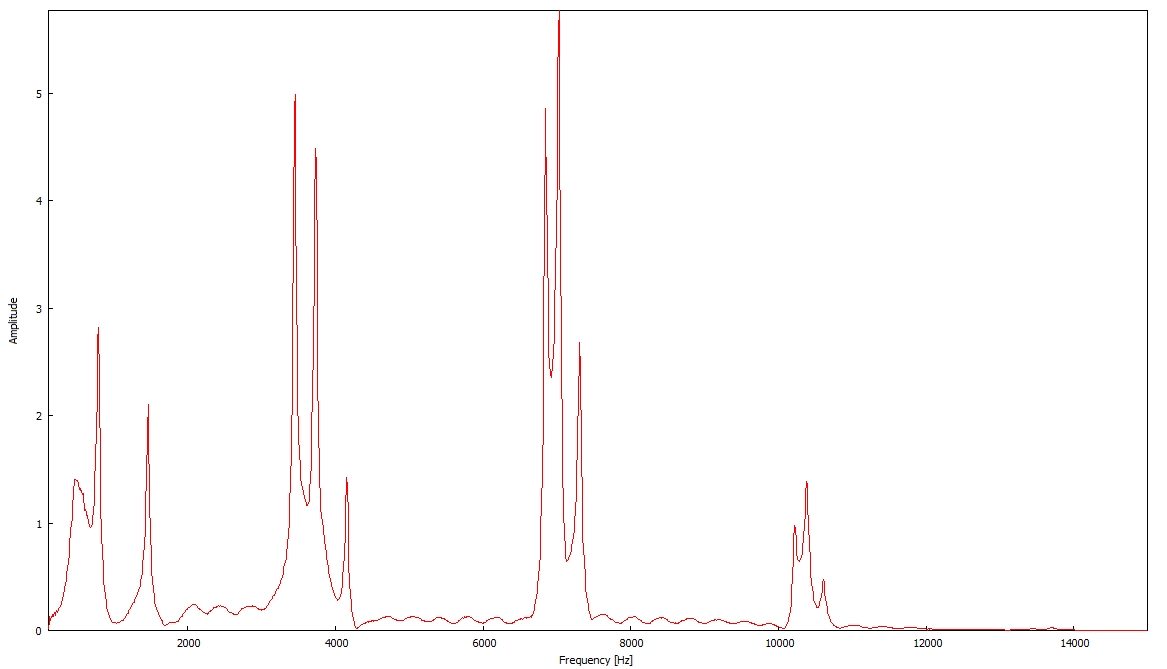
\includegraphics[width=\textwidth]{content/messungen/Chapter4b/4b_4_3_10.jpg}
\caption{Spektrum zwischen 0.1~kHz und 15~kHz einer Anordnung bestehend aus drei 50~mm langen Rohren, die durch eine Blende vom Durchmesser 10~mm getrennt sind.}
\label{fig:4b_4_3_10}
\end{figure}
\begin{figure}
\centering
\includegraphics[width=\textwidth]{content/messungen/Chapter4b/4b_4_3_13.jpg}
\caption{Spektrum zwischen 0.1~kHz und 15~kHz einer Anordnung bestehend aus drei 50~mm langen Rohren, die durch eine Blende vom Durchmesser 13~mm getrennt sind.}
\label{fig:4b_4_3_13}
\end{figure}
\begin{figure}
\centering
\includegraphics[width=\textwidth]{content/messungen/Chapter4b/4b_4_3_16.jpg}
\caption{Spektrum zwischen 0.1~kHz und 15~kHz einer Anordnung bestehend aus drei 50~mm langen Rohren, die durch eine Blende vom Durchmesser 16~mm getrennt sind.}
\label{fig:4b_4_3_16}
\end{figure}
Es ist gut zu erkennen, wie sich die schon bei zwei Rohren zu sehenden Bänder weiter aufsplitten; Nun in 3 Niveaus pro Band.
Genau wie bei zwei Rohren sorgt ein größerer Blendendurchmesser für größere Abstände zwischen zwei Energieniveaus.
Eine ähnliche Anordnung wird nun mit 4 bzw. 6 Rohren betrachtet.
Die zugehörigen Spektren sind in den Abbildungen \ref{fig:4b_4_4_10} bis \ref{fig:4b_4_6_16} zu finden.
Hier zeigen sich die gleichen Unterschiede, die oben schon beschrieben wurden.
Die Anzahl der Energieniveaus pro Band entspricht genau der Anzahl der Rohre und mit zunehmendem Blendendurchmesser wächst der Abstand zwischen zwei Energieniveaus des gleichen Bandes.
Dies führt auch dazu, dass die Bänder mit zunehmendem Blendendurchmesser näher zusammen rücken.
Auch bei gleichem Blendendurchmesser, aber steigender Anzahl an Einheitszellen verringert sich die Bandbreite.
\begin{figure}
\centering
\includegraphics[width=\textwidth]{content/messungen/Chapter4b/4b_4_4_10.jpg}
\caption{Spektrum zwischen 0.1~kHz und 12~kHz einer Anordnung bestehend aus vier 50~mm langen Rohren, die durch eine Blende vom Durchmesser 10~mm getrennt sind.}
\label{fig:4b_4_4_10}
\end{figure}
\begin{figure}
\centering
\includegraphics[width=\textwidth]{content/messungen/Chapter4b/4b_4_4_13.jpg}
\caption{Spektrum zwischen 0.1~kHz und 12~kHz einer Anordnung bestehend aus vier 50~mm langen Rohren, die durch eine Blende vom Durchmesser 13~mm getrennt sind.}
\label{fig:4b_4_4_13}
\end{figure}
\begin{figure}
\centering
\includegraphics[width=\textwidth]{content/messungen/Chapter4b/4b_4_4_16.jpg}
\caption{Spektrum zwischen 0.1~kHz und 12~kHz einer Anordnung bestehend aus vier 50~mm langen Rohren, die durch eine Blende vom Durchmesser 16~mm getrennt sind.}
\label{fig:4b_4_4_16}
\end{figure}
\begin{figure}
\centering
\includegraphics[width=\textwidth]{content/messungen/Chapter4b/4b_4_6_10.jpg}
\caption{Spektrum zwischen 0.1~kHz und 12~kHz einer Anordnung bestehend aus sechs 50~mm langen Rohren, die durch eine Blende vom Durchmesser 10~mm getrennt sind.}
\label{fig:4b_4_6_10}
\end{figure}
\begin{figure}
\centering
\includegraphics[width=\textwidth]{content/messungen/Chapter4b/4b_4_6_10.jpg}
\caption{Spektrum zwischen 0.1~kHz und 12~kHz einer Anordnung bestehend aus sechs 50~mm langen Rohren, die durch eine Blende vom Durchmesser 10~mm getrennt sind.}
\label{fig:4b_4_6_13}
\end{figure}
\begin{figure}
\centering
\includegraphics[width=\textwidth]{content/messungen/Chapter4b/4b_4_6_10.jpg}
\caption{Spektrum zwischen 0.1~kHz und 12~kHz einer Anordnung bestehend aus sechs 50~mm langen Rohren, die durch eine Blende vom Durchmesser 10~mm getrennt sind.}
\label{fig:4b_4_6_16}
\end{figure}
\FloatBarrier
\subsection{Superstrukturen}
\label{subsec:Superstrukturen}
Jeweils zwölf 50~mm Rohre werden durch Blenden getrennt. 
Ein Mal werden an jeder Stelle die gleichen Blenden vom Durchmesser 13~mm verwendet (siehe Abbildung \ref{fig:4b_5_12}) und ein Mal werden abwechselnd 13~mm und 16~mm Blenden verwendet (siehe Abbildung \ref{fig:4b_5_12_alternating}).
\begin{figure}
\centering
\begin{subfigure}{0.65\textwidth}
\includegraphics[width=\textwidth]{content/messungen/Chapter4b/4b_5_12_13.jpg}
\subcaption{Übliches Spektrum.}
\end{subfigure}
\begin{subfigure}{0.34\textwidth}
\includegraphics[width=\textwidth]{content/Scripts/4b_5_red.jpg}
\subcaption{Resonanzfrequenzen in Abhängigkeit von der Wellenzahl in der Brillouin Zone.}
\end{subfigure}
\caption{Spektrum von 0.1~kHz bis 12~kHz einer Anordnung, bestehend aus 12 50~mm Rohren, die jeweils durch eine Blende vom Durchmesser 13~mm getrennt sind.}
\label{fig:4b_5_12}
\end{figure}
\begin{figure}
\centering
\begin{subfigure}{0.65\textwidth}
\includegraphics[width=\textwidth]{content/messungen/Chapter4b/4b_5_12_alternating.jpg}
\subcaption{Übliches Spektrum.}
\end{subfigure}
\begin{subfigure}{0.34\textwidth}
\includegraphics[width=\textwidth]{content/Scripts/4b_5_alt_red.jpg}
\subcaption{Resonanzfrequenzen in Abhängigkeit von der Wellenzahl in der Brillouin Zone.}
\end{subfigure}
\caption{Spektrum von 0.1~kHz bis 12~kHz einer Anordnung, bestehend aus 12 50~mm Rohren, die abwechselnd durch Blenden vom Durchmesser 13~mm bzw. 16~mm getrennt sind.}
\label{fig:4b_5_12_alternating}
\end{figure}
Wie aus den vorigen Messungen zu erwarten war ist in Abbildung \ref{fig:4b_5_12} ein Splitting in mehrere Energieniveaus und Bänder zu beobachten. 
Im unterschied zu niedrigeren Anzahlen der Rohre sind die Peaks, vor allem am Rand eines Bandes, nicht mehr klar zu unterscheiden.
Das abwechselnde einfügen der 16~mm Blenden sorgt dafür, dass sich die Bänder in sich selbst noch einmal splitten. 
Es kommt so zu drei Bandpaketen bestehend aus jeweils zwei Bändern.
Eine weitere Superstruktur entsteht durch abwechselndes einsetzen von 50~mm und 75~mm Rohren bei gleichem Blendendurchmesser von 16~mm. Das Spektrum solch einer Struktur mit jeweils 5 Einheitszellen ist in Abbildung \ref{fig:4b_6} dargestellt.
\begin{figure}
\centering
\begin{subfigure}{0.65\textwidth}
\includegraphics[width=\textwidth]{content/messungen/Chapter4b/4b_6.jpg}
\subcaption{Übliches Spektrum.}
\end{subfigure}
\begin{subfigure}{0.34\textwidth}
\includegraphics[width=\textwidth]{content/Scripts/4b_6.jpg}
\subcaption{Resonanzfrequenzen in Abhängigkeit von der Wellenzahl in der Brillouin Zone.}
\end{subfigure}
\caption{Insgesamt 10 Rohre, abwechselnd der Länge 50~mm und 75~mm, durch 16~mm Blenden getrennt. Das Spektrum wurde zwischen 0.1~kHz und 12~kHz genommen.}
\label{fig:4b_6}
\end{figure}
Die Bandstruktur prägt sich anders aus als in den vorigen Messungen.  
Es wird vermutet, dass sich jeweils die Energieniveaus der verschiedenen Rohrlängen separat aufspalten.
Dadurch entstehen Bänder mit 10 Niveaus, an den Stellen wo die Resonanzen beider Rohrlängen übereinander fallen, sonst 5 Niveaus je Band.
\FloatBarrier
\subsection{Defekte}
In einer Anordnung aus 12 50~mm Rohren wird eins der Rohre durch ein 75~mm Rohr ersetzt. 
Damit ist die Periodizität der Anordnung gestört.
Abbildung \ref{fig:4b_7} zeigt das Spektrum der Anordnung ohne Defekt.
\begin{figure}
\centering
\begin{subfigure}{0.65\textwidth}
\includegraphics[width=\textwidth]{content/messungen/Chapter4b/4b_7_12x50.jpg}
\subcaption{Übliches Spektrum.}
\end{subfigure}
\begin{subfigure}{0.34\textwidth}
\includegraphics[width=\textwidth]{content/Scripts/4b_7_red.jpg}
\subcaption{Resonanzfrequenzen in Abhängigkeit von der Wellenzahl in der Brillouin Zone.}
\end{subfigure}
\caption{Spektrum von 12 50~mm Rohren, die jeweils durch 16~mm Blenden getrennt sind, von 0.1~kHz bis 12~kHz.}
\label{fig:4b_7}
\end{figure}
Die Abbildungen \ref{fig:4b_7_1a} bis \ref{fig:4b_7_1c} zeigen das Spektrum der Anordnung mit einem 75~mm Defekt an verschiedenen Stellen.
\begin{figure}
\centering
\begin{subfigure}{0.65\textwidth}
\includegraphics[width=\textwidth]{content/messungen/Chapter4b/4b_7_1a.jpg}
\subcaption{Übliches Spektrum.}
\end{subfigure}
\begin{subfigure}{0.34\textwidth}
\includegraphics[width=\textwidth]{content/Scripts/4b_7_1a.jpg}
\subcaption{Resonanzfrequenzen in Abhängigkeit von der Wellenzahl in der Brillouin Zone.}
\end{subfigure}
\caption{Spektrum von 0.1~kHz bis 12~kHz, der Anordnung aus Abbildung \ref{fig:4b_7} mit einem 75~mm Defekt an der ersten Stelle.}
\label{fig:4b_7_1a}
\end{figure}
\begin{figure}
\centering
\begin{subfigure}{0.65\textwidth}
\includegraphics[width=\textwidth]{content/messungen/Chapter4b/4b_7_1b.jpg}
\subcaption{Übliches Spektrum.}
\end{subfigure}
\begin{subfigure}{0.34\textwidth}
\includegraphics[width=\textwidth]{content/Scripts/4b_7_1b.jpg}
\subcaption{Resonanzfrequenzen in Abhängigkeit von der Wellenzahl in der Brillouin Zone.}
\end{subfigure}
\caption{Spektrum von 0.1~kHz bis 12~kHz, der Anordnung aus Abbildung \ref{fig:4b_7} mit einem 75~mm Defekt an der elften Stelle.}
\label{fig:4b_7_1b}
\end{figure}
\begin{figure}
\centering
\begin{subfigure}{0.65\textwidth}
\includegraphics[width=\textwidth]{content/messungen/Chapter4b/4b_7_1c.jpg}
\subcaption{Übliches Spektrum.}
\end{subfigure}
\begin{subfigure}{0.34\textwidth}
\includegraphics[width=\textwidth]{content/Scripts/4b_7_1c.jpg}
\subcaption{Resonanzfrequenzen in Abhängigkeit von der Wellenzahl in der Brillouin Zone.}
\end{subfigure}
\caption{Spektrum von 0.1~kHz bis 12~kHz, der Anordnung aus Abbildung \ref{fig:4b_7} mit einem 75~mm Defekt an der siebten Stelle.}
\label{fig:4b_7_1c}
\end{figure}
Die Spektren der mit einem 25~mm Defekt versehenen Anordnungen sind in den Abbildungen \ref{fig:4b_7_2a} bis \ref{fig:4b_7_2c} zusehen.
\begin{figure}
\centering
\begin{subfigure}{0.65\textwidth}
\includegraphics[width=\textwidth]{content/messungen/Chapter4b/4b_7_2a.jpg}
\subcaption{Übliches Spektrum.}
\end{subfigure}
\begin{subfigure}{0.34\textwidth}
\includegraphics[width=\textwidth]{content/Scripts/4b_7_2a.jpg}
\subcaption{Resonanzfrequenzen in Abhängigkeit von der Wellenzahl in der Brillouin Zone.}
\end{subfigure}
\caption{Spektrum von 0.1~kHz bis 12~kHz, der Anordnung aus Abbildung \ref{fig:4b_7} mit einem 25~mm Defekt an der ersten Stelle.}
\label{fig:4b_7_2a}
\end{figure}
\begin{figure}
\centering
\begin{subfigure}{0.65\textwidth}
\includegraphics[width=\textwidth]{content/messungen/Chapter4b/4b_7_2b.jpg}
\subcaption{Übliches Spektrum.}
\end{subfigure}
\begin{subfigure}{0.34\textwidth}
\includegraphics[width=\textwidth]{content/Scripts/4b_7_2b.jpg}
\subcaption{Resonanzfrequenzen in Abhängigkeit von der Wellenzahl in der Brillouin Zone.}
\end{subfigure}
\caption{Spektrum von 0.1~kHz bis 12~kHz, der Anordnung aus Abbildung \ref{fig:4b_7} mit einem 25~mm Defekt an der elften Stelle.}
\label{fig:4b_7_2b}
\end{figure}
\begin{figure}
\centering
\begin{subfigure}{0.65\textwidth}
\includegraphics[width=\textwidth]{content/messungen/Chapter4b/4b_7_2c.jpg}
\subcaption{Übliches Spektrum.}
\end{subfigure}
\begin{subfigure}{0.34\textwidth}
\includegraphics[width=\textwidth]{content/Scripts/4b_7_2c.jpg}
\subcaption{Resonanzfrequenzen in Abhängigkeit von der Wellenzahl in der Brillouin Zone.}
\end{subfigure}
\caption{Spektrum von 0.1~kHz bis 12~kHz, der Anordnung aus Abbildung \ref{fig:4b_7} mit einem 25~mm Defekt an der siebten Stelle.}
\label{fig:4b_7_2c}
\end{figure}
Ein relevanter Unterschied zwischen den Abbildungen ist nur in den Amplituden zu erkennen. 
Es scheint kein Messbarer Einfluss des Defekts auf den Aufbau zu entstehen.